\documentclass[11pt, spanish]{report}
\usepackage[spanish]{babel}
\usepackage{amsmath}
\selectlanguage{spanish}
\usepackage[utf8]{inputenc}
\usepackage[a4paper, top=2.50cm, bottom=2.50cm, left=2.50cm, right=2.50cm]{geometry}

\usepackage{etoolbox}
\patchcmd{\chapter}{\thispagestyle{plain}}{\thispagestyle{fancy}}{}{}

% Quotes
\usepackage[autostyle]{csquotes}

% Times New Roman font (use on the entire report)
\usepackage{times}

% Last page
\usepackage{lastpage}

% Links to reference
\usepackage[colorlinks=false, hidelinks]{hyperref}  

% Footer
\usepackage{fancyhdr}
\fancyhf{}
\pagestyle{fancy}
% delete header line
\renewcommand{\headrulewidth}{0pt}
% right footer
\rfoot{pág. \thepage\ de \pageref{LastPage}}

% Interlineado
\renewcommand{\baselinestretch}{1.5}

% Distancia entre párrafos
\setlength{\parskip}{6pt}

% Para usar el símbolo R (Reales), por ejemplo
\usepackage{amssymb}

% Carpeta de imágenes
\usepackage{graphicx}
\usepackage{caption,subcaption}% http://ctan.org/pkg/{caption,subcaption}
\graphicspath{{images/}}

% Lib: Matrices con índices (labels)
\usepackage{libs/kbordermatrix}% http://www.hss.caltech.edu/~kcb/LaTeX.shtml
\newcommand{\noindex}{\hspace*{-0.8em}}%

\bibliographystyle{apalike}

% Título
\title{
	{\huge \textsf{Sistemas de Recuperación de Información}}\\
	{\Large \textbf{Universidad Nacional de Rosario}}\\
	{\Large Facultad de Ciencias Exactas, Ingeniería y Agrimensura}\\
	{\large Licenciatura en Ciencias de la Computación}\\
	{\large {\itshape Bases de Datos Avanzadas}} \\
}

\author{Luciano Perezzini \and Estanislao Ruiz Sorazábal}
\date{2016}


\begin{document}
	\maketitle
	
	\chapter*{Resumen}
		En el presente trabajo realizaremos una revisión en el campo de la recuperación de información, tomando la definición y el concepto de los compatriotas que han estado estudiando e investigando en el área durante años, para luego poder analizar algunas de las etapas del proceso que realizan los sistemas de recuperación de información: el procesamiento y la indexación de los documentos, los modelos más influyentes para la implementación de estos sistemas abordando la representación de los objetos de información y la forma de recuperar esos objetos ante una consulta, así como también algunas medidas que nos permitan determinar la calidad de la recuperación que tiene un sistema. \par

Además un poco de historia sobre la Web y algunos conceptos y algoritmos desarrollados para analizar, recolectar, indexar, recuperar y visualizar información de esa gran red de redes. Donde se deben lidiar con problemas extras como la heterogeneidad de los datos y la generación de información de fuentes poco confiables.\par

Por último un acercamiento a los sistemas recomendadores que tratan de recuperar información relevante para cada usuario y ponerla a su disposición mediante el uso de diversas herramientas y algoritmos. Estas aplicaciones son utilizadas en nuestras vidas cotidianas, cada vez, con más frecuencia.

	
	% Indice
	\tableofcontents
	
	\chapter{Introducción}
		\section{Recuperación de Información}
	La recuperación de información ocupa un gran área de interés en las Ciencias de la Computación. Brinda herramientas las cuales utilizamos de forma cotidiana y que, en ciertas situaciones, dependemos en su totalidad. Estas herramientas nos acercan de forma eficaz a información de nuestro interés. Cabe destacar que, sin el desarrollo y la existencia de ésta rama, los usuarios comunes y corrientes no serían capaces de obtener la información que necesitan dado el tamaño de las fuentes de información que va en aumento día a día. Existen diversas definiciones de recuperación de información; una breve pero contundente descripción es la siguiente: \textit{La recuperación de información trata con la representación, almacenamiento, organización y acceso a ítems de información tales como documentos, páginas Web, catálogos online, datos estructurados y no estructurados, objetos multimedia. La representación y organización de los ítems de información tienen que ser tales como para proveer a los usuarios un fácil acceso a información de su interés} \cite{baeza1999}.
	
	\subsection{Recuperación de Información vs. Recuperación de Datos}
	Dada una consulta del usuario que representa el input necesario de un sistema de recuperación de información, el objetivo principal de éste es darle al usuario acceso rápido a un conjunto de documentos con información útil ordenados de acuerdo a su relevancia.  \\
	Por otro lado un sistema de recuperación de datos sólo se encarga de determinar el conjunto de documentos que cumple cierta proposición sobre los datos del documento.
	En el primer caso, el problema es más complejo porque además de saber como recuperar los objetos de información se tiene que determinar cuales objetos resultarán más importantes que otros para el usuario de acuerdo a los términos utilizados en la consulta, los cuales tienen cierta ambigüedad derivada del lenguaje natural, debido a esto la respuesta tendrá un grado de imprecisión y es posible que se recuperen parcialmente los documentos que el usuario considera importantes. \\
	En cambio la respuesta de un sistema de recuperación de datos es exacta de acuerdo a la consulta que se le realiza. En la mayoría de los casos utilizando lenguajes altamente estructurados que lo vuelve mucho más sensible a los errores que pueda haber en el input del usuario.
	
	\subsection{El proceso de recuperación y \textit{ranking}}
		Supongamos que tenemos una colección de documentos de la cual, un usuario, quiere obtener información relevante. Los sistemas de recuperación de información deben, primeramente, procesar estos documentos: eliminar palabras \textit{stop--words}, \textit{stemming}, \textit{normalización}, entre otras. Este proceso se conoce, generalmente, como \textbf{procesamiento de documentos} y se analiza detalladamente en el Capítulo XX. Resumiendo, este proceso tiene como finalidad extraer \textit{términos} para, luego, crear un índice. Estos términos se consideran palabras claves (\textit{keywords}) dentro de la colección. \par

		Una vez que se extraen los términos de los documentos, se procede a crear un índice del texto. Para ésto, se utilizan diferentes estructuras de datos; pero la más popular es llamada \textbf{índice invertido}. Esta tarea se denomina \textit{indexado} y debe ser realizada \textit{offline}, antes de que el sistema de recuperación de información pueda procesar cualquier consulta. La implementación de éste proceso es de extrema importancia; ya que, dadas largas colecciones de documentos, computarlo puede tomar tiempo considerable. \par

		Ahora, teniendo la colección de indexada documentos, el proceso de recuperación de información puede comenzar. Este consiste, básicamente, en que el usuario ingresa al sistema una consulta; la cual estará escrita en lenguaje natural o en uno cercano muy cercano. A continuación, el sistema aplica una serie de procedimientos de análisis de texto a la consulta. Estos procedimientos son similares a los que se realizan en el procesamiento de texto anterior: eliminación de \textit{stop--words}, correcciones de errores de ortografías, entre otros. Es decir se le extraen los términos como en los documentos. El sistema puede presentar al usuario consultas sugeridas, para que el mismo confirme. Una vez procesada la consulta, el sistema recupera un conjunto de documentos. Estos documentos contienen los términos que han sido extraídos de la consulta ingresada por el usuario. Obtener éstos documentos es una tarea rápida ya que fueron indexados previamente. El proceso anterior es llamado \textit{proceso de recuperación}. \par

		Luego de realizar el proceso de recuperación, se deben ordenar los documentos dentro del conjunto obtenido. En la efectividad de esta tarea se encuentra en juego la conformidad del usuario y el feedback del mismo al sistema. Este ordenamiento se realiza mediante funciones de similitud, las cuales se detallan en el Capítulo 4.

	\chapter{Procesamiento de Texto}
		Los cuatro grandes pasos para la construcción de un índice invertido:
\begin{enumerate}
	\item Recolectar los documentos a ser indexados.
	\item Realizar el proceso \textit{tokenization} al texto.
	\item Realizar un procedimiento linguistico sobre los \textit{tokens} obtenidos en el paso anterior.
	\item Indexar a cada \textit{token} con los documentos en los cuales aparece.
\end{enumerate}

En éste capítulo desarrollaremos los primeros tres pasos de la enumeración anterior; es decir, veremos cómo, a partir de una colección de documentos, extraer \textit{tokens} de los textos y luego realizarles un procedimiento linguístico para obtener los términos (\textit{keywords}) que, finalmente, serán indexados.

\section{Obteniendo la secuencia de caracteres en un documento}
	Típicamente, los documentos a ser indexados son bytes en un archivo o en un servidor web. El primer paso en el procesamiento de documentos es convertir éstas secuencias de bytes en una secuencia de caracteres. Este suele ser un procedimiento complicado ya que se debe determinar en qué esquema de codificación están codificadas las secuencias de caracteres, como por ejemplo Unicode UTF-8 o varios estándares comerciales. Para determinar el esquema en cuestión se utilizan procedimientos de Machine Learning, métodos heurísticos o utilizando metadata especificada en el documento mismo. Una vez que el esquema es determinado, se decodifica la cadena de bytes obteniendo así una cadena de caracteres.
	
\section{Determinando el vocabulario de términos}
	\subsection{\textit{Tokenization}}
		Dada una secuencia de caracteres, \textit{tokenization} es la tarea de cortarla en pedazos, llamados \textit{tokens}, y también, quizás al mismo tiempo, deshechar ciertos caracteres tales como aquellos de puntuación, \cite{manning2009}. Veamos un ejemplo:
		\begin{quote}
			Entrada: Friends, Romans, Countrymen, lend me your ears; \\
			Salida: \fbox{Friends} \fbox{Romans} \fbox{Countrymen} \fbox{lend} \fbox{me} \fbox{your} \fbox{ears}
		\end{quote}
		
		Veamos las siguientes definiciones. Un \textit{token} es una instancia de una secuencia de caracteres. Un \textit{tipo} es la clase de todos los tokens que contienen la misma secuencia de caracteres. Un \textit{término} es un tipo probablemente normalizado el cual está incluido en el diccionario del sistema de recupereación de información. Estos últimos derivan de tokens aunque procesados por distintas técnicas de normalización que se detallarán más adelante. Como ejemplo, si el documento a ser indexado es \textit{to sleep perchance to dream}, luego habrá 5 tokens pero sólo 4 tipos (ya que existen dos instancias de la palabra \textit{to}), y por lo tanto 4 términos.
		
		Durante el proceso de \textit{tokenization} suele haber distintas dificultades dependiendo del idioma del texto. Es decir, muchas veces se debe elegir qué tokens utilizar. En un caso \enquote{normal} se procede de manera trivial: se toma la secuencia de caracteres de entrada, se identifican espacios en blanco, se \textit{cortan} y se deja de lado signos de puntuación; de ésta forma obtenemos los tokens. Pero no todo es tan fácil. Por ejemplo, el idioma inglés suele representar ciertos problemas: ¿qué se debe hacer con el uso de los apóstrofes?. Veamos el siguiente documento:
		\begin{quote}
			Mr. O'Neill thinks that the boys' stores about Chile's capital aren't amusing.
		\end{quote}
		
		Tomando la palabra \textit{O'Neill}, existen diferentes formas de \textit{tokenization}. Pero, ¿cuál consideramos como la \enquote{correcta}?:
		\begin{quote}
			\begin{ttfamily}
				\fbox{neill} \\
				\fbox{oneill} \\
				\fbox{o'neill} \\
				\fbox{o'} \fbox{neill} \\
				\fbox{o} \fbox{neill} \\
			\end{ttfamily}
		\end{quote}
		
		Lo mismo sucede, en el documento anterior, con la palabra \textit{aren't}. Veamos:
		\begin{quote}
			\begin{ttfamily}
				\fbox{aren't} \\
				\fbox{arent} \\
				\fbox{are} \fbox{n't} \\
				\fbox{aren} \fbox{t} \\
			\end{ttfamily}
		\end{quote}
		
		Elegir ciertas posibilidades como \enquote{correctas} puede traer distintas consecuencias. Una consulta booleana como \texttt{neill AND capital} será exitosa en tres casos pero no en los otros tres. Razonablemente, para consultas booleanas como también para consultas de lenguaje natural (\textit{free--text queries}) se requiere que se realice exactamente el mismo procedimiento de \textit{tokenization} de documentos y consultas. Esto se hace, generalmente, procesando consultas con el mismo \textit{tokenizer}. \par
		
		Las Ciencias de la Computación ha introducido nuevas cadenas de caracteres las cuales un \textit{tokenizer} debería devolverlas como un solo token; éstas, por ejemplo, son: direcciones de e--mail, URLs, direcciones numéricas de IP, y más. Una posibildad es omitir de los índices las cadenas anteriores, pero resultaría una gran desventaja para aquellos usuarios del sistema de recuperación de información no poder buscar por éstas cadenas. \par
		
		Cortar palabras mediante espacios en blanco puede dividir aquellas secuencias de caracteres las cuales deben ser consideradas como un solo token. Esto ocurre generalmente con nombres (\textit{Santa Fe, Argentina}), números de teléfonos y fechas (\textit{24 de mayo de 2016}). Esto puede resultar en una mala recuperación de información. \par
		
		Resumiendo, cada idioma trae diferentes \enquote{problemas} en cuanto a cómo debe realizarse el proceso de \textit{tokenization}. Algunos idiomas presentan mayores dificultades que otros. Por lo tanto, una forma de sortear éstas dificultades es mediante una técnica denominada \textit{Identificación de Lenguaje}. Esta técnica usa modelos de \textit{Machine Learning} para reconocer específicos patrones en la secuencia de caracteres y así, finalmente, identificar el idioma.
		
	\subsection{\textit{Stop words}}
		Se denominan \textit{stop words} aquellas palabras que son extremadamente comunes y que no aportan un valor significativo a la hora de indexar documentos. Estas palabras son excluidas totalmente del vocabulario de términos. Para ejemplificar, a continuación se nombran algunas de las \textit{stop words} del idioma español:
		\begin{quote}
			\begin{ttfamily}
				un \\
				desde \\
				cierto \\
				ir \\
				vamos \\
				tiene \\
				es				
			\end{ttfamily}
		\end{quote}
		
		La forma de determinar una lista de \textit{stop words} es ordenando los términos, de un documento, mediante frecuencia de términos (es decir, el número total de veces cada que término aparece en un documento) y luego quitar de la lista aquellos más frecuentes. Una vez que se completa la lista de \textit{stop words}, sus términos son descartados a la hora de indexar los documentos dentro de la respectiva colección. Descartar \textit{stop words} de una colección de documentos, reduce notablemente el número de \textit{postings} que el sistema de recuperación de información debe almacenar. \par
		
		Muchas veces, descartar \textit{stop words} puede lograr que el sistema no recupere la información que verdaderamente estamos buscando. Un ejemplo de lo anterior puede ser la consulta \texttt{vuelos a Buenos Aires}: si aquí, el sistema, descarta la palabra \texttt{a} (la cual es un textit{stop word}) se tendrá como consulta resultante \texttt{vuelos Buenos Aires}. El sistema, ante una consulta así, no nesariamente devolverá aquellos vuelos que se dirigan a Buenos Aires, sino también aquellos vuelos que salen desde Buenos Aires; perdiendo el significado de la consulta original. Otras determinadas consultas se ven afectadas. Entre ellas, títulos de canciones y versos que  consisten, comúnmente, en \textit{stop words}. Ejemplificando lo anterior, una frase de William Shakespear: textit{To be or not to be}. \par
		
		En los primeros sistemas de recuperación de información las listas de \textit{stop words} eran considerablemente largas: entre 200 y 300 términos. Luego, con el tiempo, éstas listas fueron disminuyendo (de 7 a 12 términos) hasta, finalmente, no utilizarlas. Los motores de búsqueda en la Web, por lo general, no utilizan listas de \textit{stop words}: utilizando buenas técnicas de compresión se reducen los costos de almacenamiento de \textit{postings} de palabras comunes.
		
	\subsection{Normalización de tokens}
		Hasta ahora, hemos detallado el proceso de documentos en una colección de la siguiente forma:
		\begin{enumerate}
			\item Se toma como entrada un documento: un archivo de bytes.
			\item Se convierte la secuencia de bytes anterior en una secuencia de caracteres.
			\item Se toma la secuencia de caracteres anterior y se le realiza el procedimiento llamado \textit{tokenization}: se divide en \textit{partes} para obtener tokens.
		\end{enumerate}
		Sin embargo, muchas veces resulta que existen dos secuencias de caracteres que no son sintácticamente iguales pero que significan lo mismo y se quiere que, obviamente, indexen los mismos documentos. Por ejemplo, si un usuario busca la palabra \textit{USA} éste espera que el sistema de recuperación de información devuelva documentos los cuales contiene el término \textit{USA} como también \textit{U.S.A}. \par
		
		La normalización de tokens es el proceso de canonizar tokens con el objetivo de \textit{igualar} términos a pesar de algunas diferencias en sus secuencias de caracteres, \cite{manning2009}. Existen diversos métodos de normalización de tokens. Entre ellos, el método  mas estándar, es crear clases de equivalencias, que son nombradas por alguno de los miembros de las clases. Como ejemplo, tomemos los tokens \texttt{anti-discriminatorio} y \texttt{antidiscriminatorio}. Utilizando el método anterior, se creará una clase de equivalencia llamada, por ejemplo, \textit{antidiscriminatorio} y \enquote{almacenará} los dos tokens anteriores; luego, las búsquedas por uno de los términos devolverá documentos que contienen el otro término, y viceversa. \par
		
		A continuación se presentan algunas formas de normalización que son comúnmente implementadas por sistemas de normalización de tokens. En muchos casos éstas técnicas pueden llegar a ser muy útiles pero tambien dañinas.
		\begin{itemize}
			\item \textbf{Signos diacríticos}. El español es uno de los idiomas en los cuales se utilizan éstos símbolos. Un signo diacrítico es un signo gráfico que confiere a los signos escritos (no necesariamente letras) un valor especial. Entre ellos se encuentran los acentos ortográficos (\ \' \ ) y (\ \` \ ), la diérisis (\ \" \ ), la virguililla de la \textit{ñ} y la coma (,), entre otros. En un sistema de recuperación de información querremos que el mismo, ante una consulta como \texttt{películas} y \texttt{pelicula}, devuelvan exactamente los mismos documentos; es decir, que el sistema discrimine el acento ortográfico. Esto puede realizarse normalizando tokens eliminando los signos diacríticos. Lo anterior puede causar problemas, ya que muchas veces los signos diacríticos asignan significados a ciertas palabras. Por ejemplo, en el idioma español, \textit{peña} no significa lo mismo que \textit{pena}. Sin embargo, no siempre se debe prestar atención a la lingüística del idioma, sino a cómo los usuarios escriben sus consultas. Estos, generalmente, las escriben omitiendo signos diacríticos por razones de velocidad o hábitos. En éstos casos, la respuesta es igualar todas las palabras a aquellas sin diacríticos.
			\item \textbf{Conversión a minúsculas}. Esta estrategia sugiere convertir todas las letras de una palabra a minúsculas. Por lo general es una muy buena estrategia, ya que igualará  términos como, por ejemplo, \texttt{iPod} a \texttt{ipod}. Aunque, también, ésta estrategia puede provocar incidentes. Por ejemplo, en el idioma inglés, si un usuario ingresa como consulta la palabra \texttt{US} (acrónimo de \textit{United States}) el sistema la igualará con la palabra \texttt{us} la cual quiere decir \textit{nosotros}. Por lo tanto, no sólo recuperará información acerca del país Estados Unidos. Una alternativa para solucionar éstos inconvenientes es transformar a minúsculas sólo determinadas letras dentro de una palabra. La heurística más simple es convertir a minúsculas palabras que se encuentren en el comienzo de una oración y todas aquellas palabras que ocurren en un título (por lo general se encuentran en mayúsculas por cuestión de diseño). 
		\end{itemize}
		
	\subsection{\textit{Stemming} y \textit{Lemmatization}}
		Ahora, no todos los documentos utilizan palabras de la misma forma; aunque, al fin y al cabo, quieran decir -- interpretar -- lo mismo. Por ejemplo: \textit{acción}, \textit{accionar}, \textit{accionando}. Razonablemente, pretendemos que todo sistema de recuperación de información, al buscar cualquiera de éstas palabras, devuelva aquellos documentos que también cotengan otras palabras derivadas. \par
		
		Según \cite{manning2009}, \textit{Stemming} usualmente refiere a procesos heurísticos que \enquote{cortan} los finales de palabras. Mientras que \textit{Lemmatization} usualmente refiere a realizar estudios morfológicos a palabras con el propósito de eliminar finales flexivos para retornar la forma base de las mismas, llamada \textit{lemma}. Siguiendo el ejemplo de \cite{manning2009}, si se encuentra con la palabra \textit{saw}, del idioma inglés, \textit{stemming} probablemente devolverá sólo \textit{s}, mientras que \textit{lemmatization} intentará devolver \textit{see} ó \textit{saw} dependiendo si el token se utiliza como verbo o sustantivo. \par
		
		\textit{Stemming} y \textit{lemmatization} son realizados con la ayuda de componentes adicionales de software que son agregados al proceso de indexado. Existen numerosos componentes de software libre, entre ellos: \cite{multiLemmatisation} y \cite{Snowball} \par
		
		Entre los diversos métodos de \textit{stemming} se encuentra un algoritmo escrito en 1979 en Cambridge (Inglaterra) por el Dr. Martin Porter. El algoritmo es comúnmente conocido como \textbf{Porter \textit{stemmer}} y es el \textit{stemmer} más popular para el idioma inglés. \par
		El algoritmo de Porter consiste en 5 fases de reducción de palabras aplicadas secuencialmente, las cuales no se detallarán aquí en su totalidad. De \cite{porterSpammer}, la primera fase aplica las siguientes reglas:
		\begin{quote}
			\textbf{Regla} \\
			SSES $\rightarrow$ SS \\
			IES $\rightarrow$ I \\
			SS $\rightarrow$ SS \\
			S $\rightarrow$  \\
			donde '$\rightarrow$' indica \enquote{reemplazar}.
		\end{quote}
		Como ejemplo de cada una de las reglas anteriores, veamos:
		\begin{quote}
			\textbf{Ejemplo} \\
			carasses $\rightarrow$ caress \\
			ponies $\rightarrow$ poni \\
			caress $\rightarrow$ caress \\
			cats $\rightarrow$ cat \\
		\end{quote}
		
		Ahora, en vez de utilizar un \textit{stemmer}, es posible utilizar un \textit{lemmatizer}. Estos son herramientas de procesamiento de lenguaje natural las cuales hacen un análisis morfológico completo de palabras para determinar sus correspondientes \textit{lemmas}. Realizar éstos análisis proveen beneficios para la recuperación de información. \par
		
		Utilizar un \textit{stemmer} ó un \textit{lemmatizer} puede traer diversos problemas para ciertos idiomas en algunos casos. Es decir, reemplazar un \textit{stemmer} por un \textit{lemmatizer} ó un \textit{lemmatizer} por un \textit{stemmer} no necesariamente soluciona los problemas.
					
		
	\chapter{Indexado}
		%% Indexing and searching de Baeza
% - Introducción.
% - Cómo construir índices invertidos (la estructura de datos más usada para construir un índice
%	sobre documentos en una colección.
% - Más...

\section{Introducción}

El propósito de crear y mantener un índice es optimizar la recuperación de documentos relevantes a partir de una consulta de búsqueda. Con lo cual un sistema de recuperación sin un índice necesitaría revisar todos los documentos de la colección en cada consulta lo que demandaría demasiado tiempo y poder de cómputo. El espacio necesario para almacenar el índice como el tiempo necesario para actualizarlo es compensado por este ahorro de tiempo ante cada respuesta del sistema. \par

Se denomina indexación al procedimiento de construir un índice invertido de los términos del contenido sobre la colección de documentos. Esta estructura relaciona cada término con la lista de postings que contiene la referencia de los documentos en donde ocurre al menos una vez ese término. \\
Es llamado también índice booleano ya que solo puede determinar si un término aparece en un documento o no, sin dar a conocer detalles como, por ejemplo, la posición en el documento o la cantidad de ocurrencias. Los índices están relacionado con la forma que tiene la representación de los documentos aún así consideramos que las contrucciones habituales de índices utilizan palabras.\par


\section{Construcción del índice}

Con el próposito de mejorar la velocidad de respuesta, algunos factores que se pueden evaluar en el diseño y construcción de un índice serán el tamaño de almacenamiento del índice, velocidad de consulta, costo de mantenimiento, tolerancia a fallas, costo de fusionar índices, entre otros.
Para obtener los términos (keywords) de cada documento es necesario realizar el procedimiento detallado en el capítulo 2 y así obtener un conjunto más reducido de palabras a indexar. \\
Un índice invertido consiste de un conjunto de palabras o términos (vocabulario) que normalmente se mantiene en memoria principal y una lista de ocurrencia de los términos en la colección de documentos (posting list).\\
La estructura que representa el vocabulario puede ser una lista, árbol de búsqueda o tabla hash. Cada una de éstas tiene un costo de búsqueda, inserción y borrado asociado lo cual dependerá de lo que se considere más importante a la hora de elegir la estructura de datos a utilizar.\\

\section{Comparación con otros índices}
La estructura de índice invertido es considerada la más eficiente para realizar búsqueda de documentos basados en texto en colecciones de cualquier tamaño. \\
Otra clase de índices orientados a palabras son los archivos de firma (signature files) que minimizan la sobrecarga de procesamiento utilizando funciones hash pero realizando una búsqueda secuencial sobre el índice que lo hace adecuado para colecciones pequeñas de documentos. \\
Una alternativa a utilizar cuando el vocabulario es gigantesco son los árboles de sufijos que permiten buscar cadenas de texto de manera veloz con un alto costo de almacenamiento asociado y para que realmente sea eficiente deberá trabajar en memoria principal.
		
	\chapter{Modelos de Recuperación de Información}
		%% Introducción sobre Modeling en IR de Baeza
% - Introducción.
% - Taxonomía.
% - Carecterización formal de modelos IR.

\section{Modelo booleano}
	El modelo booleano es el modelo más simple dentro de los que puede implementar un sistema de recuperación de información. Para desarrollarlo, presentamos el siguiente ejemplo. Supongamos que se tiene a disposición las obras del poeta inglés William Shakespear llamada \textbf{Shakespear's Collected Works}. Supongamos también que queremos saber qué obras, dentro de la colección, contiene las palabras Brutus, Caesar pero no Calpurnia. Una forma de resolver la consulta anterior es la siguiente: supongamos que para cada documento (obra dentro de la colección \textbf{Shakespear's Collected Works}) si contiene o no cada una de las palabras que Shakespear utilizó al escribir las obras (Shakespear usó cerca de 32000 palabras diferentes). El resultado es una matriz llamada \textbf{matriz de incidencia término--documento}: $(t, d)$ es igual a 1 si y sólo si el documento en la columna $d$ contiene el término de la fila $t$, y es igual a 0 en caso contrario. La que sigue es parte de la matriz en cuestión tomando el ejemplo de la colección de obras de William Shakespear:
	\begin{quote}
		\[
		\kbordermatrix{
					& Antony \ and \ Cleopatra 	& Julius \ Caesar 	& 	The \ Tempest & 	Hamlet 	& Othello 	& Macbeth 	& ... \\
		Antony		&	1					&		1		&		0		&	0		&	0		&	1		& \\
		Brutus		&	1					&		1		&		0		&	1		&	0		&	0		& \\
		Caesar		&	1					&		1		&		0		&	1		&	1		&	1		& \\
		Calpurnia	&	0					&		1		&		0		&	0		&	0		&	0		& \\
		Cleopatra	&	1					&		0		&		0		&	0		&	0		&	0		& \\
		mercy		&	1					&		0		&		1		&	1		&	1		&	1		& \\
		worser		&	1					&		0		&		1		&	1		&	1		&	0		& \\
		...			&						&				&				&			&			&			&
		}
		\]
	\end{quote}
	
	Dependiendo de la forma en que observamos la matriz término--documento es posible obtener un vector para cada término, el cual indica los documentos en los cuales aparece, ó un vector para cada documento, el cual muestra los términos que ocurren en él. \par
	
	Ahora, resolvamos la consulta del principio; es decir, recuperar todas aquellas obras de la colección que contiene las palabras Brutus, Caesar pero no Calpurnia. Podemos representar ésta consulta de forma booleana, de forma muy simple, de la siguiente manera: \texttt{Brutus AND Caesar AND NOT Calpurnia}. Luego, tomamos los vectores de \texttt{Brutus}, \texttt{Caesar} y el complemento de \texttt{Calpurnia} y los operamos:
	\begin{quote}
		\begin{ttfamily}
			110100 AND 110111 AND 101111 = 100100
		\end{ttfamily}
	\end{quote}
	El resultado anterior nos indica que los documentos los cuales satisfacen la consulta anterior son \textit{Antony and Cleopatra} y \textit{Hamlet}. \par
	
	El \textbf{\textit{modelo booleano}} es un modelo de recuperación de información en el cual podemos plantear cualquier consulta que se encuentre en forma de una expresión booleana de términos; es decir, en la cual los términos estén combinados con operadores AND, OR, y NOT, \cite{manning2009}. El modelo representa a cada documento como un conjunto de palabras.
	
	\subsection{Utilizando un índice invertido}
		Supongamos que tenemos una colección con 1 millón de documentos y que cada documento tenga alrededor de 1000 palabras. Típicamente, habrá alrededor de 500 mil términos distintos en cada uno de éstos documentos. Las dimensiones anteriores varían respecto a diferentes colecciones, pero nos dan una idea de los problemas que tendremos que solucionar utilizando una matriz de incidencia término--documento. Tomando la suposición anterior, debemos construir una matriz término--documento de dimensión 500K $\times$ 1M: ésta posee medio trillón de 0's y 1's, demasiados para caber en la memoria de una computadora estándar. \par
		
		Una representación mucho mejor es sólo recordar los términos que ocurren; es decir, sólo las posiciones 1's. Esto nos lleva a la definición de índice invertido que se desarrolló anteriormente en el Capítulo 2: mantenemos un \textit{diccionario} de términos, luego, para cada término, una lista que guarda en qué documentos el término ocurre. Cada ítem de la lista anterior es llamado \textit{posting}; éste guarda el ID del documento. \par
		
		Para ganar beneficios de rapidez, el sistema de recuperación de información debe contruir el índice invertido antes de que un usuario realice una consulta. Se deben desarrollar los siguientes pasos:
		\begin{enumerate}
			\item Recolectar los documentos a ser indexados.
			\item Convertir cada documento en una lista de tokens (\textit{Tokenization}).
			\item Realizar precedimientos lingüísticos a la lista de tokens del paso 2 (\textit{Normalization}). De ésta forma se obtienen tokens normalizados los cuales, finalmente, serán los términos a indexar.
			\item Indexar aquellos documentos en los cuales ocurren los términos obtenidos en el paso 3 creando un índice invertido.
		\end{enumerate}
		Los pasos 1--3 consisten en el procesamiento de textos que se desarrolló en el capítulo anterior. Mientras que la implementación del índice invertido (paso 4 de la lista anterior) se estudió en el Capítulo 2.
		
		% Figura 1.4 (manning2009)
		
		\subsection{Procesamiento de una consulta booleana}
			Ahora, utilizando índices invertidos como estructura más eficiente para indexar documentos en un sistema de recuperación de información, ¿cómo procesamos una consulta booleana?. Consideremos la siguiente consulta en el modelo booleano sobre el índice invertido presentado en la figura anterior:
			\begin{quote}
				\begin{ttfamily}
					Brutus AND Calpurnia
				\end{ttfamily}
			\end{quote}
			El sistema ejecuta los siguientes pasos:
			\begin{enumerate}
				\item Localizar \texttt{Brutus} en el diccionario de términos.
				\item Devolver sus \textit{postings}.
				\item Localizar \texttt{Calpurnia} en el diccionario de términos.
				\item Devolver sus \textit{postings}.
				\item Intersectar las listas de \textit{postings} de los pasos 2 y 4.
			\end{enumerate}
			Como resultado final, tenemos que la consulta en cuestión se satisface en los documentos 2 y 31 como bien se muestra a continuación:
			\begin{quote}
				\begin{tabular}{lll}
					Brutus & $\longrightarrow$ & \fbox{1}$\rightarrow$\fbox{2}
												$\rightarrow$\fbox{4}
												$\rightarrow$\fbox{11}
												$\rightarrow$\fbox{31}
												$\rightarrow$\fbox{45}
												$\rightarrow$\fbox{173}
												$\rightarrow$\fbox{174} \\
					Calpurnia & $\longrightarrow$ & \fbox{2}$\rightarrow$\fbox{31}
												$\rightarrow$\fbox{54}
												$\rightarrow$\fbox{101} \\
					Intersección & $\Longrightarrow$ & \fbox{2}$\rightarrow$\fbox{31}
				\end{tabular}
			\end{quote}
			
		\subsection{El modelo booleano ante modelos de \textit{ranking} de relevancia}
			Dada una colección de documentos $D$. Sean $d_j \in D$ y $q$ una consulta. Por lo aprendido anteriormente, el documento $d_j$ será relevante ante la consulta $q$ si o sólo si los términos contenidos en la representación del documento en cuestión hacen verdadera a la expresión booleana de la consulta $q$. A lo anterior se lo llama \textit{ranking} de un documento $d_j$ ante una consulta $q$, y lo notamos $R(d_j,q)$. Claramente, es un \textit{ranking} booleano y es la principal desventaja del modelo booleano ante otros modelos de recuperación de información más complejos: las consultas booleanas sólo devuelven un conjunto de documentos el cual no es posible ordenar ya que todos son igual de importantes. \par
			
			Por lo tanto, nos encontramos con un modelo simplista e imposible de satisfacer ciertas necesidades como, por ejemplo:
			\begin{itemize}
				\item Poder escribir consultas en lenguaje natural en vez de en álgebra booleana, la cual sólo tienen conocimientos científicos de la información.
				\item Podríamos tener, también, la necesidad de realizar consultas de \enquote{proximidad} como por ejemplo \texttt{Gates NEAR Microsoft}. Para realizar ésto, el índice tiene que tener la capacidad de capturar proximidades de términos en documentos.
				\item El modelo booleano sólo almacena la presencia o ausencia de un término, pero comúnmente qusieramos acumular evidencia, dando más \enquote{peso} (importancia) a documentos quienes contienen un determinado término varias veces en contraposición a aquellos quienes los contienen una sóla vez. Para realizar ésto debemos tener un método para obtener la frecuencia de un término en un documento en listas de \textit{postings}.
				\item Poder ordenar, en orden de relevancia, los documentos que devuelve el sistema ante una determinada consulta escrita por un usuario.
			\end{itemize}
			
			Las necesidades anteriores se satisfacen en modelos de \textit{ranking} de relevancia como se desarrollarán en las próximas secciones. Es decir, en aquellos modelos de recuperación de información los cuales la función \textit{ranking}, $R$, que emplean no es binaria, como la que emplea el modelo booleano.

\section{Modelo vectorial}

En ciertos contextos el uso de una asignación binaria en la importancia de un documento resulta muy limitante por eso surgió un modelo que permite realizar coincidencias parciales entre una consulta y los documentos de la colección. \\

En este modelo, documentos y consultas se representan mediante vectores t dimensionales, donde t es el número total de términos. Cada componente del vector representa un peso que será asignado al término correspondiente en el documento o la consulta. \\

Formalmente, Sea $k_{i}$ un término indexado del conjunto $V$ de términos, $d_{j}$ un documento en $D$ y $w_{i,j}$  el peso asociado a $(k_{i},d_{j})$ entonces definimos el vector $\overrightarrow{d_{j}}= (w_{1,j}, w_{2,j}, … , w_{t,j})$. De manera análoga se representan las consultas. \\  

Los pesos  asignados a los términos indexados son usados para computar el grado de similitud entre cada documento con la consulta que realiza usuario. Luego se ordenan los documentos recuperados de acuerdo a su relevancia, representada por la distancia entre los vectores de los documentos con el vector de la consulta.\\
\subsection{Ponderación de términos} 

Se asocia un peso a cada término que aparece en el documento $d_{j}$. Si un término no aparece tendrá peso igual a 0. Este peso cuantifica la importancia del término indexado en la descripción del contenido en el documento $d_{j}$.\\

Hay diferentes formas de asignar los pesos teniendo en cuenta que no todos los términos son igualmente descriptivos para un documento.\\

Algunas propiedades de los términos indexados resultan útiles para evaluar su importancia sobre el documento. Para modelos clásicos de IR se suponen que los pesos de los términos son independientes entre sí. En resumen, la cantidad de veces que ocurre un término no está relacionado con la cantidad de veces que pueda aparecer otro.\\

Tomaremos como ejemplo de factor de ponderación de términos: TF-IDF (Frecuencia de término - Frecuencia inversa de documento) es el producto de dos estadísticas que busca reflejar la importancia del término sobre un documento de la colección. Un término es mas importante que otro en un documento si este es más representativo de la información que contiene el documento que aquel. De esta forma, un término es proporcional a la frecuencia con la que ocurre pero ante términos con la misma frecuencia tendrá mayor ponderación el que aparezca en la menor cantidad de documentos, buscando capturar así la idea de especificidad del término. \\


\[ w_{i,j} =
  \begin{cases}
    (1 + \log{f_{i,j}}) \times \log{\frac{N}{n_{i}}} & \quad \text{if } f_{i,j} > 0\\
    0  & \quad \text{otro caso}\\
  \end{cases}
\]

%				\begin{figure}[h]
%					\includegraphics[width=8cm]{tf-idf}
%					\centering
%					\caption{Función de asignación de pesos}
%				\end{figure}

\subsection{Función de ranking}

Tomando el esquema de asignación de ponderación TF-IDF, el peso de cada término influirá en el ranking de documentos de acuerdo a su especificidad. \\ 

Dada una consulta y un documento con una única coincidencia pero en un término de mayor peso, éste podría darle más valor de ranking que otro documento con varias coincidencias en términos de menores peso. \\

Entonces podemos calcular la similitud entre dos documentos o entre un documento y una consulta como el coseno del ángulo formado por los vectores representativos de cada documento dj y la consulta q. 

				\begin{figure}[h]
					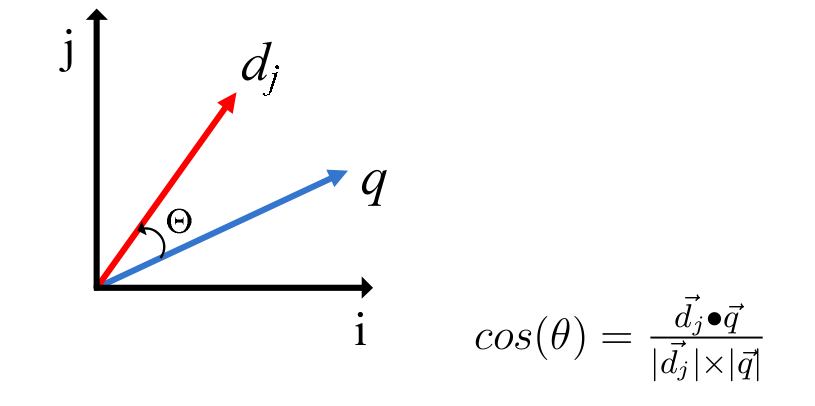
\includegraphics[width=8cm]{vector-distance}
					\centering
					\caption{Calcular la similitud}
				\end{figure}


\section{Modelo probabilístico}

Este modelo intenta resolver el problema de la recuperación de información estimando la probabilidad de que un documento sea relevante ante una determinada consulta.\\
Se representa a los documentos como vectores de incidencia de términos. Inicialmente se asignan pesos binarios a los términos dependiendo si está presente o no en el documento.\\
Se supone que existe para cada consulta un conjunto de respuesta ideal $R$ que satisface la consulta, no se lo conoce de antemano pero se va refinando consulta tras consulta.\\
La consulta inicial del usuario permite al sistema responder con un primer conjunto de respuesta. Luego el usuario inspeccionará algunos documentos y el sistema utilizará esa información para mejorar la descripción del conjunto de respuesta. Iterando este procedimiento se espera obtener una caracterización lo mas parecida a la descripción del conjunto de respuesta ideal.\\
Para este modelo se asume la hipótesis del principio de probabilidad donde dada una consulta $q$ y un documento $d_{j}$, el modelo probabilístico estimará la probabilidad que el usuario encuentre relevante al documento $d_{j}$ asumiendo que la probabildad de relevancia sólo depende de la consulta y la representación del documento en el modelo.\\

\subsection{Funcion de ranking}

Como ya dijimos, la ponderación de los términos indexados es binaria, es decir, $w_{i,j} \in {0,1}$.
Sea $R$ el conjunto de respuesta conocido como relevante para la consulta del usuario. Definimos $\overline{R}$ como el complemento de $R$ y sea $P(R|\overrightarrow{d_{j}})$ la probabilidad que el documento $\overrightarrow{d_{j}}$ resulte relevante a la consulta $q$ y $P(\overline{R}|\overrightarrow{d_{j}})$ la probabildad de que $d_{j}$ no sea relevante a la consulta $q$.\\
La similaridad entre el documento $\overrightarrow{d_{j}}$ y la consulta $q$ queda definida por la función:

			\begin{equation}
				sim(\overrightarrow{d_{i}},j) = \frac{P(R | \overrightarrow{d_{j}})}{P(\overline{R} | \overrightarrow{d_{j}})}
			\end{equation}	
				
Usando la regla de Bayes y sabiendo que $P(R)$ y $P(\overline{R})$ valen lo mismo para todos los documentos de la colección:

			\begin{equation}
				sim(\overrightarrow{d_{i}},j) = \frac{P(R | \overrightarrow{d_{j}}) \times P(R,q)}{P(\overline{R} | \overrightarrow{d_{j}}) \times P(\overline{R},q)} \sim  \frac{P(\overrightarrow{d_{j}} | R, q)}{P( \overrightarrow{d_{j}} | \overline{R}, q)}
			\end{equation}	
				


\section{Comparación entre modelos}

Partiendo del modelo booleano que es el más simple pero también básico porque no tenemos la posibilidad de realizar coincidencias parciales lo que define una baja performance del sistema respecto de los otro dos modelos que logran una recuperación de informarción ordenada por el grado de relevancia. \\
En cuanto a los últimos dos modelos, como se menciona en \cite{baeza1999}, Croft sugiere que el modelo de probabilidades aporta un mejor rendimiento de recuperación. Sin embargo, se demostró que el rendimiento del modelo vectorial supera a los demás para colecciones de documentos más generales.\\
En contraste podemos considerar el hecho que en estos modelos se asume independecia entre los términos, es decir que en ningún caso se considera una correlación entre ellos.

		
	\chapter{Evaluación}
		%% Retrieval Evaluation de Baeza
% - Introducción.
% - Retrieval performance.
% - Más...

Conociendo que ante la consulta de un usuario que presenta cierto grado de incertidumbre, la lista de documentos recuperados no será una respuesta exacta y determinística como ocurre en sistemas de bases de datos relacionales. Las medidas de evaluación propias de una sistema de recuperación de información nos permiten conocer la calidad de las respuestas del sistema ante determinadas consultas. Más allá de las medidas de rendimiento de cualquier sistema computacional, como el tiempo de respuesta o el espacio necesario para responder una consulta, que también se podrán tener en cuenta. \\

En este capítulo haremos foco sobre medidas específicas en la recuperación de información. Es importante mencionar que cuando se quiere medir la performance de un sistema hay que tener en claro la tarea de recuperación que realiza, la cual podrá consistir de consultas procesadas por lote (batch mode) o sino mediante una sesión interactiva donde el usuario irá especificando la información que necesita a través de una serie de pasos. Esta aclaración es para ilustrar que existen diferentes formas de procesamiento con lo cual la manera de evaluar su rendimiento también será diferente. \\

Muchas medidas de rendimiento y correctitud fueron propuesta, sólo veremos las tres que consideramos mas interesantes pero sepan que hay muchas más que se pueden aplicar quizás dependiendo el contexto en donde se utilice el sistema, para mas información puede consultar \cite{baeza2011} \\

Consideremos una consulta \textit{q} sobre una colección de documentos \textit{D} y una estrategia de recuperación \textit{S} a evaluar. Suponemos conocido el conjunto \textit{R} de documentos determinados como revelantes para el usuario ante la necesidad de información que representa la consulta \textit{q}, en este caso los documentos se clasifican como relevantes o no, en otro escenario es posible que la relevancia sea multivaluada. \\ \\ \\
Sea \textit{A} el conjunto ordenado de respuesta de un sistema aplicando la estrategia \textit{S} sobre la consulta \textit{q}, mientras que \textit{R} es el conjunto de todos los documentos de información revelantes para esa consulta.

	\begin{figure}[h]
		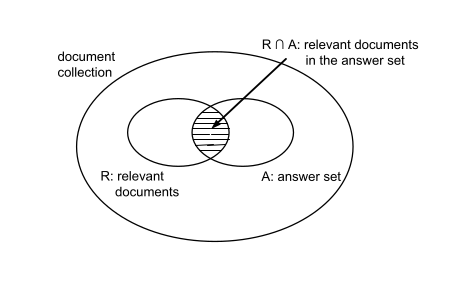
\includegraphics[width=8cm]{evaluation-retrieval}
		\centering
		\caption{Diagrama de conjuntos. (Figura extraída de \cite{baeza2011})}
	\end{figure}

\section{Precisión}
Esta medida define la fracción de los documentos recuperados que son relevantes para el usuario cuando realiza la consulta \textit{q}. Podemos considerar que cada documentos relevante recuperado es un acierto (hit) del sistema. \\

					\begin{equation}
						Precision = \cfrac{|R \cap A|}{|A|}
					\end{equation}
	
\section{Recall o Exhaustividad}
Esta medida define la proporción de los documentos relevantes que fueron recuperados para la consulta \textit{q}. Cada documento relevante no recuperado representa un desacierto (miss) del sistema. \\

					\begin{equation}
						Recall = \cfrac{|R \cap A|}{|R|}
					\end{equation}
					
Con esta dos medidas podemos definir una curva donde nos muestre el valor de precisión alcanzado por el sistema utilizando \textit{S} para ciertos valores de exhaustividad. \\
	
\section{Fall-out o Proporción de fallos}
La proporción de fallos define la fracción de los documentos no relevantes que fueron recuperados para una consulta. Representa la tasa de falsos positivos en el sistema.\\
Resulta deseable minimizar esta variable o maximizar la exhaustividad y al mismo tiempo lograr mayor precisión en las respuestas. \\
Siendo \textit{N} el tamaño de la colección de los documentos, podemos definir el índice de fallos como sigue:

					\begin{equation}
						Fall-out = \cfrac{|A - (R \cup A)|}{N - |R|}
					\end{equation}

%---Hablar sobre las medidas online y la diferencia con las medidas offline
		
	\chapter{Buscando en la Web}
		Podemos considerar a la World Wide Web (o sólo Web) como una colección de páginas web (documentos) la cual crece y se modifica día a día. En este capítulo se desarrollan conceptos sobre cómo tratar a la Web, al ser tan diferente de todos las colecciones tradicionales anteriormente vistas.

\section{Historia}
	Como bien se detalló anteriormente, la Web no tiene precedentes en diversas cuestiones:
	\begin{itemize}
		\item En escala.
		\item En la falta de coordinación a la hora de su desarrollo.
		\item En la diversidad de sus participantes.
	\end{itemize}
	Esto hace que recuperar información en la Web sea más complicado que recuperar información en colecciones de documentos tradicionales. \par
	
	Veamos, de forma resumida, cómo es el funcionamiento de comunicación entre un \textit{cliente} y un \textit{servidor}:
	\begin{quotation}
		Un \textit{cliente} tal como un \textit{browser}; es decir, una aplicación con interfaz gráfica que renderiza el contendido de código HTML recibido mediante una petición a un servidor web. El \textit{browser} especifica una URL (\textit{Universal Resource Locator}) como, por ejemplo \texttt{http://www.google.com.ar/intl/en/policies/terms/regional.html}. La cadena de caracteres \texttt{http} refiere al protocolo que se debe usar para transmitir datos (HTTP, por \textit{HyperText Transfer Protocol}). El segmento \texttt{google.com.ar} refiere al dominio y especifica la raíz de la jerarquía de páginas web. \texttt{/intl/en/policies/terms/regional.html} indica la ruta en donde se encuentra el recurso, en este caso un archivo HTML \texttt{regional.html} que será retornado por el servidor web con el cual el \textit{cliente} interactuará. En este archivo, también, se encuentran los \textit{links}. Este procedimiento es clave a la hora de obtener el contenido de una página web (texto e \textit{hyperlinks}) para indexar documentos
	\end{quotation}
	
	El hecho de que los \textit{browsers} fueron y son capaces de mostrar al usuario el código HTML detrás de una página web, hizo que muchos desarrolladores, aprendieran cómo estaban implementadas aquellas páginas que consideraban modelos y, así, implementaran las suyas. De esta manera, el número de páginas en la Web comenzó a incrementar y a convertirse en un espacio en donde cualquier persona, con algunos pocos conocimientos informáticos, pudiese comunicarse y expresarse ante millones de personas alrededor del planeta. De repente, la Web se convirtió en la mejor opción a la hora de obtener y proveer información. \par
	
	Toda la información que contiene la Web resulta de poca utilidad si no se poseen herramientas para descubrir y recuperar información. Lo más importante es que éstas herramientas estén al alcanze de usuarios \textit{comunes} que navegan la red a través de un web \textit{browser}; y deben ser lo más simples posibles. Por lo tanto, los científicos e investigadores tomaron noción de la desventaja anterior y comenzaron a desarrollar los buscadores web. Los primeros intentos se podían dividir en dos categorías:
	\begin{itemize}
		\item Motores de búsquedas de indexación de texto tales como Altavista, Excite y Infoseek. Consistía en consultas escritas en lenguaje natural (o muy cercano al mismo) utilizando índices invertidos y mecanismos de \textit{ranking} tales como se detalló en capítulos anteriores.
		\item Utilizando taxonomías. En éste caso, se le presentaba al usuario un \textit{árbol} jerárquico el cual él mismo debía recorrer hasta llegar a la página deseada. Esto tiene grandes desventajas, veamos:
			\begin{itemize}
				\item Clasificar páginas web en categorías es, prácticamente, un trabajo manual. Por lo tanto, es difícil de escalar con el tamaño de la Web.
				\item Sólo se deben categorizar las \textit{mejores} páginas web y dejar de lado las demás. Ahora, ¿qué se considera como una \textit{buena} página web?.
			\end{itemize}
	\end{itemize}
	Dadas las desventajas anteriores, la popularidad de las taxonomías disminuyó con el tiempo. Una de las grandes empresas que las implementaba en su buscador era Yahoo!. \par
	
	Como se detalló anteriormente, implementar buscadores utilizando taxonomías era \textit{exponencialmente} ineficiente. Por lo tanto, se siguió estudiando cómo utilizar las técnicas de recuperación de información tradicionales; es decir, aquellas que implementan índices invertidos y funciones de relevancia para ordenar documentos, teniendo en cuenta el gran volúmen de documentos en la Web. Los primeros motores de búsqueda contenían índices con millones de páginas. Estos fueron satisfactorios para indexar una gran parte de la Web en ese momento, pero no eran eficiente a la hora de rankear los documentos por relevancia. Por lo tanto, para controlar la calidad de las páginas se necesitaron nuevos mecanismos y técnicas de recuperación de información basados en la teoría tradicional que estuvimos viendo de los sistemas de recuperación de información.
	
\section{Características de la Web}
	Publicar en la Web se convirtió en un medio de democratización disponible para millones de personas. Con lo cual, crear contenidos, ahora, no solo es tarea de editores bien entreanados sino también de millones de personas con acceso a Internet. Esto conlleva a preguntarse cuánto podemos confiar en los contenidos disponibles en diversas páginas web. La democratización en la creación de contenidos convirtió rápidamente a la Web en un medio que contiene verdades, falsedades y contradicciones. De esto, nace la siguiente pregunta: \textit{¿en qué páginas debemos confiar?}. Esta es una pregunta difícil de responder ya que para ciertas personas, algunos editores pueden ser confiables como otros pueden no serlo. Cómo un motor de búsqueda web debe calcular esta medida de \textit{confianza} para cada página web y eso es lo que buscaremos desarrollar a lo largo de éste capítulo. Esto es de suma importancia ya que, para los usuarios finales de la Web, un motor de búsqueda es la única vía para recuperar información entre todo el contenido disponible.
	
\subsection{\textit{Web Graph}}
	Según \cite{manning2009}, podemos dividir las páginas web en \textbf{estáticas} o \textbf{dinámicas}. Se consideran estáticas aquellas donde su contenido no varía de un pedido para ésa página a la siguiente. Un profesor que manualmente mantiene su propia página web, se considera estática. Mientras que las dinámicas son mecánicamente generadas por una aplicación que reside en uno o varios servidores en respuesta a consultas sobre bases de datos. \par
	
	Sabemos que una forma de definir un grafo consiste en dar su conjunto de nodos y aristas; así \cite{manning2009} define al \textit{web graph} de la siguiente forma:
	\begin{itemize}
		\item El conjunto de nodos es igual al conjunto de todas las páginas web HTML estáticas pertenecientes a la Web.
		\item Se considera como una arista dirigida a todo \textit{hyperlink} que \enquote{conecta} una página web a otra página web.
	\end{itemize}
	El \textit{web graph} no es fuertemente conexo: existen pares de páginas web las cuales es imposible proseguir desde una página del par hacia la otra siguiendo \textit{hyperlinks}. Se definen como \textbf{in--links} a aquellos \textit{hyperlinks} que \enquote{salen} desde una página web y \textbf{out--links} a aquellos que \enquote{llegan} a una página web.
	
	%% figura 19.3 de manning2009
	\begin{figure}[h]
		\includegraphics[width=8cm]{small-web-graph}
		\centering
		\caption{\textit{Web graph} en el cual existen seis páginas web. La página web posee 3 \textit{out--links} y 1 \textit{in--link}}
	\end{figure}
	
\section{La experiencia de usuario en un buscador web}
	Como se ha descripto anteriormente, la búsqueda de información en la Web cambia de forma significante con respecto a los sistemas de recuperación tradicionales. En éstos últimos, los usuarios debían ser profesionales en el arte de formular las búsquedas; es decir, debían tener entrenamiento desde cómo escribir una consulta (por ejemplo, una consulta \textit{booleana}) hasta tener un buen conocimiento en cómo estaban estructurados los documentos dentro de la colección. En contraste, los usuarios de sistemas de recuperación de información en la Web tienden a no conocer cómo las páginas están estructuradas y cómo se debe escribir una consulta. En resumen, los motores de búsqueda no deben imponer éstas restricciones ya que, al fin y al cabo, sus usuarios no son profesionales en el campo de la recuperación de información. \par
	
	Claramente, cuanto más tráfico un motor de búsqueda pueda atraer, tendrá más ganancia económica con respecto a las búsquedas patrocinadas. Por lo tanto, ¿cómo hacen los motores de búsquedas para lograr lo anterior?. Del gran éxito de Google, podemos aprender lo siguiente:
	\begin{itemize}
		\item Enfoque en \textit{precisión} en vez de en \textit{recall} en los primeros resultados.
		\item Interfaz gráfica de usuario simple, liviana y con pocos elementos gráficos. Es decir, una interfaz en donde el texto sea el elemento gráfico más importante. Esto hace que la experiencia sea totalmente \textit{responsive} sin esperar demasiado tiempo en cargar los resultados de la búsqueda.
	\end{itemize}
	
	Según \cite{manning2009}, las consultas que los usuarios pueden realizar en un buscador web pueden tener diversos propósitos y se pueden clasificar en los siguientes tres:
	\begin{itemize}
		\item \textit{Consultas de información}. Son aquellas las cuales buscan recuperar información sobre algún tema en particular (como por ejemplo, una enfermedad) y, en general, no existe una única página web la cual contiene toda la información necesaria.
		\item \textit{Consultas de navegación}. En éstas, los usuarios buscan la página web oficial de alguna entidad (por ejemplo, Apple): esperan que el primer resultado que devuelva el motor de búsqueda resulte ser la mismísima página de la entidad en cuestión. Suele suceder que hay usuarios no buscan información adicional sobre la entidad más de la que aparece en el \textit{homepage} oficial.
		\item \textit{Consultas de transacción}. El objetivo de esta clase de consultas es realizar una transacción, de algún tipo, en la Web: tales como comprar un producto, descargar un archivo, realizar una reserva y demás. En éstos casos, el usuario espera que el motor de búsqueda retorne páginas web que presten los servicios mencionados.
	\end{itemize}
	
	Decidir en cuál categoría subyace una determinada consulta puede ser un gran reto.
	
\section{\textit{Web crawling}}
	\subsection{Introducción}
		\enquote{\textit{Web crawling} es el proceso por el cual se recogen páginas de la Web, con el motivo de indexarlas y apoyar un motor de búsqueda}, \cite{manning2009}. Su objetivo es recoger el número máximo de páginas útiles, junto con la estructura de \textit{links} que las interconectan, de forma rápida y eficiente. \par
		
		El foco de ésta sección es detallar el funcionamiento de un \textit{web crawler}, también llamado \textit{web spider}.
		
		%% figura 19.7 (manning2009) 
		
	\subsection{Características que un \textit{crawler} debe proporcionar}
		\begin{itemize}
			\item \textbf{Robustez}. En la Web, existen servidores los cuales crean los denominados \textit{spider traps}; éstos son generadores de páginas web que engañan a los \textit{crawlers} logrando que los últimos extraigan información de infinitas páginas web dentro de un determinado dominio. Luego, los \textit{crawlers} deben ser lo suficientemente inteligentes como para sortear los \textit{spider traps}. Cabe destacar que no siempre éstas \enquote{trampas} son maliciosas: muchas veces son el resultado de carencia de profesionalismo en el desarrollo de páginas web.
			\item \textbf{Cortesía}. Los servidores web especifícan de forma implícita y también explícita políticas las cuales regulan cada  \enquote{cuánto} un \textit{crawler} puede visitarlos. Estas políticas se deben respetar.
		\end{itemize}
	
	\subsection{Características que un \textit{crawler} debería proporcionar}
		\begin{itemize}
			\item \textbf{Distribución}. El \textit{crawler} debería tener la posibilidad de ejecutarse en máquinas distribuidas.
			\item \textbf{Escalable}. La arquitectura del \textit{crawler} debería ser lo más práctica posible como para poder extenderse y escalar su frecuencia de rastreo añadiendo más hardware y ancho de banda.
			\item \textbf{\textit{Performance} y eficiencia}. El sistema de \textit{crawling} debería utilizar de forma eficiente recursos de sistemas como ancho de banda, procesador, almacenes de datos, y demás.
			\item \textbf{Calidad}. El \textit{crawler} debería procesar, primero, aquellas páginas de la Web que sean \enquote{útiles}.
			\item \textbf{Frescura}. Aquellas páginas web las cuales son devueltas por un motor de búsqueda deberían estar actualizadas. Por lo tanto, el \textit{crawler} debe procesar páginas con una frecuencia que se aproxime a la frecuencia con la cual páginas web modifican su contenido.
			\item \textbf{Extensibilidad}. La aquitectura de los \textit{crawlers} deberían ser modulares. Eso permite que éstos puedan adaptarse con nuevas tecnologías de datos, nuevos protocolos de extracción de información, y demás.
		\end{itemize}
		
	\subsection{Funcionamiento de un \textit{crawler}}
		Veamos en qué consiste el funcionamiento básico de un \textit{web crawler}. El \textbf{crawler} comienza con un conjunto inicial, también llamado \textit{conjunto semilla}, que contiene uno o más URLs. Toma un URL de éste conjunto, extrae el texto y sus \textbf{links} (los cuales apuntan a otra página web). El texto que se extrae de cada página web es enviado a un indexador de texto. Los URLs de los \textit{links} que se extrayeron son enviados a un conjunto llamado \textit{frontera de URLs}; el cual contiene URLs los cuales todavía deben ser procesados por el \textit{crawler}. En el comienzo, el conjunto \textit{frontera de URLs} contiene sólo al \textit{conjunto semilla}. La tarea del \textit{crawler} es procesar cada uno de los URLs pertenecientes al conjunto \textit{frontera de URLs}. Una vez que esos URLs son procesados, nuevamente se colocan en el conjunto \textit{frontera} con el objetivo de que se extraiga información actualizada de los mismos, ya que, muy probable y razonablemente el contenido de las páginas web cambie con el tiempo.
		\subsubsection{Arquitectura}
			Un sistema de \textit{crawling} demanda de múltiples módulos, como muestra la Figura \ref{fig:crawler-architecture}. Veamos los más importantes:
			\begin{enumerate}
				\item El conjunto \textit{frontera}, que contiene URLs los cuales aún tienen que ser procesado por el \textit{crawler}.
				\item Un módulo de resolución de DNS el cual, dado un URL, determina el servidor en el cual se encuentra y, por lo tanto, en el cual el \textit{crawler} debe extraer la información.
				\item Un módulo que utiliza el protocolo \texttt{http} para \enquote{devolver} la página web de una determinado URL.
				\item Un módulo que \enquote{parsea} el texto y el conjunto de \textit{links} extraidos de una página web.
				\item Un módulo que determina si un determinado \textit{link} ya ha sido procesado por el \textit{crawler} y si existen \textit{links} duplicados dentro del conjunto \textit{frontera}.
			\end{enumerate}
			
			%% figura 20.1 (manning2009)
			\begin{figure}[h]
				\includegraphics[width=8cm]{crawler-architecture}
				\centering
				\caption{Arquitectura de un web \textit{crawler}}
				\label{fig:crawler-architecture}
			\end{figure}
			
		\subsubsection{\textit{Robots Exclusion Protocol}}
			Muchas veces se quiere que ciertas páginas de un cierto dominio, no sean alcanzables por un determinado \textit{crawler}; es decir, que éste no las procese. Para lograr eso los desarrolladores web (\textit{webmasters}) colocan un archivo, llamado \texttt{robots.txt}, en la raíz de la jerarquía. El protocolo se denomina \textit{Robots Exclusion Protocol}. \par
			
			Veamos un ejemplo de archivo \texttt{robots.txt} el cual especifica que ningún \textit{crawler} (también llamado \textit{agente}) no debe visitar los URLs cuya posición en el archivo de jerarquía comienza con \texttt{/yoursite/temp}, excepto por el \textit{crawler} \enquote{searchengine}:
			\begin{quote}
				\begin{ttfamily}
					User-agent: * \\
					Disallow: /yoursite/temp/ \\ \\
					
					User-agent: searchengine \\
					Disallow:
				\end{ttfamily}
			\end{quote}
			
			Este archivo debe ser extraido desde el sitio web con el fin de comprobar si el URL en cuestión satisface las restricciones, y puede, por lo tanto, ser añadido al conjunto \textit{frontera de URLs}.
			

\section{Análisis de \textit{links}}
	Dada una consulta de usuario en un buscador web, éste debe rankear las páginas web que obtiene como respuesta en función de su \textit{importancia} para el usuario. Una de las técnicas comúnmente usadas por los motores de búsquedas web es el \enquote{análisis de \textit{links} }, cuyo objetivo es computar un puntaje a una página web dada cualquier consulta. \par
	
	El análisis de \textit{links} está \enquote{inspirado} en el análisis de citación, el cual se utiliza en el área conocida como bibliometría. El análisis de citación busca, resumidamente, cuantificar la influencia (\enquote{importancia}) de artículos escolares analizando el patrón de citaciones entre ellos. El análisis de \textit{links} en la Web trata a los \textit{hyperlinks} que lleva de una página web hacia otra página web como una \enquote{atribución de autoridad}; es decir, si una página $A$ desarrolla un tema en particular y añade un \textit{link} $l$, para obtener más información sobre el tema, el cual apunta a otra página web $B$, implícitamente, la página $A$ le concede autoridad sobre el tema en cuestión a la página $B$. \par
	
	Cabe destacar que, simplemente reconocer la importancia de una página web mediante el número de \textit{in-links} que posee no es buena idea: por ejemplo, personas mal intencionadas pueden crear otras páginas conteniendo \textit{links} que apunten a una página en particular la cual se quiere que obtenga más relevancia para ubicarse en los primeros puestos en respuesta a determinadas búsquedas en la Web. El ejemplo anterior se conoce como \textit{link spam}. \par
	
	En ésta sección desarrollaremos ideas básicas sobre el uso del \textit{web graph} en el análisis de \textit{links} detallando un método de análisis de \textit{links} en particular: PageRank.
	
	\subsection{Conceptos básicos}
		La siguiente figura representa dos páginas web $A$ y $B$ donde, en $A$, existe un \textit{link} el cual apunta a $B$. El análisis de \textit{links} se basa en dos conceptos:
		\begin{enumerate}
			\item El \textbf{anchor text} que apunta a la página $B$ es una buena descripción sobre qué trata $B$.
			\item El \textit{link} de $A$ hacia $B$ representa una \enquote{ratificación} de la página $B$, por el creador de $A$. Esto no siempre ocurre; por ejemplo, muchas páginas web de empresas poseen, en cada página de su dominio, punteros (\textit{links}) hacia notas de copyright. El análisis de \textit{links} descarta aquellos \textit{links}.
		\end{enumerate}
		
		%% figura 19.2 (manning2009)
		
		Veamos el siguiente \textit{link}, el cual apunta a la página web del \textit{Journal of the ACM}:
		\begin{quote}
			\begin{ttfamily}
				<a href="http://www.acm.org/jacm/">Journal of the ACM</a>
			\end{ttfamily}
		\end{quote}
		Aquí su correspondiente \textit{anchor text} es \textit{Journal of the ACM} y, claramente, describe el contenido de la página web \texttt{http://www.acm.org/jacm/}. \par
		
		El uso de \textit{anchor texts} puede ser explotado por motores de búsqueda. Por ejemplo, los términos de los \textit{anchor texts} pueden ser incluidos como términos bajo los cuales indexar la página web destino, indicando que éstos términos ocurren como \textit{anchor texts} en lugar de términos dentro de la página. Por lo tanto, los \textit{postings} para el término \texttt{computer} incluirá el documento \texttt{http://www.ibm.com}, \texttt{http://www.apple.com}, entre otros. \par
		
		Los \textit{anchor texts}, también, pueden utilizarse para producir \textit{spam}: un página web puede autoreferenciarse creando \textit{anchor texts} apuntando a si mismo para lograr más relevancia ante ciertas consultas de términos. Este tipo de \textit{spam} es combatido y detectado por motores de búsqueda.
		
	\subsection{PageRank}
		PageRank es un método de análisis de \textit{links} introducido por Google. El objetivo de éste método es asignar a cada página web del \textit{web graph} un puntaje numérico entre 0 y 1. A éste puntaje se lo conoce como su \textit{PageRank}. El PageRank de un nodo dependerá de la estructura de \textit{links} del \textit{web graph}. Un motor de búsqueda, dada una consulta, computa para cada página web un puntaje el cual es la combinación de cientos de métodos como la similitud del coseno y proximidad de términos, junto con el puntaje que otorga el método PageRank. \par
		
		Idea:
		\begin{quote}
			\begin{itshape}
				\enquote{Consideremos un usuario de la Web que comienza en una determinada página (un nodo del web graph) y comienza una caminata aleatoria en la Web como sigue. En cada paso, el usuario procede desde su actual página web A hacia otra página B, elegida aleatoriamente, la cual A apunta mediante un hyperlink. La Figura \ref{fig:random-surfer} muestra al usuario en el nodo A. A contiene tres hyperlinks los cuales apuntan a las respectivas páginas web B, C y D. En el siguiente paso, el usuario se dirige a alguno de éstos tres nodos con probabilidad equivalentes 1/3. Mientras el usuario continúa la caminata, visitará más frecuentemente algunos nodos a comparación de otros. Intuitivamente, éstas son páginas web con un número mayor de \textbf{in--links} que otras. La idea de PageRank es que los nodos los cuales, durante ésta caminata, son frecuentemente más visitados que otros son más importantes}
			\end{itshape}, \cite{manning2009}.
		\end{quote}
		
		%% Figura 21.1 (manning2009)
		\begin{figure}[]
			\centering
			\includegraphics[width=3cm]{random-surfer}
			\caption{Un usuario aleatorio de la Web quien se encuentra en la página A.}
			\label{fig:random-surfer}
		\end{figure}
		
		
		Ahora, podemos encontrarnos con el problema en el cual el usuario se encuentra en un determinado nodo del \textit{web graph} el cual no posee \textit{out--links}. Para resolver éste problema, el método PageRank introduce una operación llamada \textit{teleport}. En ésta, el usuario \enquote{salta} desde un nodo hacia otro en el \textit{web graph}. La operación se lleva a cabo porque el usuario escribe otro URL en el \textit{browser}. Si $N$ es el número total de nodos en el \textit{web graph}, \textit{teleport} lleva al usuario a todos los nodos con probabilidad 1/$N$. \par
		
		Cuando se asigna el puntaje PageRank a cada nodo del grafo, se utiliza la operación \textit{teleport} de dos maneras:
		\begin{itemize}
			\item Cuando un nodo no contiene \textit{out--links}, el usuario invoca la operación \textit{teleport}.
			\item Cuando un nodo contiene \textit{out--links}, el usuario invoca la operación \textit{teleport} con probabilidad $0 < \alpha < 1$ y la caminata estándar anteriormente detallada con probabilidad $1 - \alpha$, donde $\alpha$ es un parámetro anteriormente elegido (por lo general, $\alpha = 0,1$).
		\end{itemize}
		
		Veremos que en el proceso combinado (caminata aleatoria más invocación de la operación \textit{teleport}) que realiza el usuario al navegar por la Web, éste visita cada nodo $v$ del \textit{web graph} una fracción fija de tiempo $\pi (v)$ la cual depende de la estructura de \textit{links} del \textit{web graph} y el valor anteriormente fijado de $\alpha$. Al valor $\pi (v)$ se lo llama \textit{PageRank} de $v$. Ahora, para poder computar ese valor debemos recordar algunos conceptos como, por ejemplo, cadenas de Markov.
		
		\subsubsection{Cadenas de Markov}
			Definición:
			\begin{quote}
				En la teoría de la probabilidad, se conoce como cadena de Markov a un tipo especial de proceso estocástico discreto en el que la probabilidad de que ocurra un evento depende \textit{solamente} del evento inmediatamente anterior. Esta propiedad recibe el nombre de \textit{propiedad de Markov}.
			\end{quote}
			
			Una cadena de Markov consiste de $N$ \textit{estados} (eventos). Para hacer una analogía con el \textit{web graph}, cada estado en una cadena de Markov corresponderá a una página web (nodo) del mismo. \par
			
			La representación de una cadena de Markov se realiza mediante una matriz $N \times N$ llamada \textit{matriz de probabilidades de transición}, la cual notamos como $P$. En ésta, se cumplen las siguientes propiedades:
			\begin{itemize}
				\item $P_{i,j} \in [0,1], \forall i,j$, y
				\item $\sum_{j = 1}^{N} P_{i,j} = 1, \forall i$.
			\end{itemize}
			La cadena de Markov puede estar en cualquiera de los $N$ estados en cualquier momento. $P_{i,j}$ nos indica la probabilidad de que la cadena de Markov, en el siguiente paso, se encuentre en el estado $j$, dado que el estado actual es $i$. Este valor se conoce como \textit{probabilidad de transición} y sólo depende del estado actual $i$. \par
			
			Veamos un ejemplo en el cual tenemos una cadena de Markov con tres estados: $A$, $B$ y $C$. En ésta, desde el estado $A$ se puede proseguir con una probabilidad de 0.5 al estado $B$ ó al estado $C$. Desde $B$ o $C$, es posible proseguir con probabilidad 1 al estado $A$. \par
			
			%% Figura 21.2 (cadena y matriz) (manning2009)
			\begin{figure}[]
				\centering
				\includegraphics[width=4cm]{markov-chain}
				
				\[
			P =
			\begin{bmatrix}
				0 & 0.5 & 0.5 \\
				1 & 0 & 0 \\
				1 & 0 & 0
			\end{bmatrix}
			\]
			
				\caption{Cadena de Markov}
			\end{figure}
			
			Un \textbf{vector de probabilidad} $N$--dimensional en el cual cada componente corresponde a uno de los $N$ estados de una cadena de Markov puede ser visto como la distribución de probabilidades sobre sus estados. La suma de los $N$ componentes del vector debe ser 1. \par
			
		\subsubsection{Utilizando cadenas de Markov en el \textit{web graph}}
			Ahora, ¿cómo podemos utilizar la teoría de la probabilidad, más específicamente cadenas de Markov, para modelar la actividad de un usuario al \enquote{navegar} por la Web?. Podemos pensar a un usuario aleatorio que navega por el \textit{web graph} como una cadena de Markov, con un estado por cada página web, y cada transición de probabilidad siendo representada por la probabilidad de moverse desde una página web hacia otra. Como es de esperar, \textbf{la operación \textit{teleport}} vista anteriormente, \textbf{contribuye en la obtención de éstas probabilidades de transición}. Notemos $A$ a la matriz de adyacencias correspondiente al \textit{web graph}; es decir, si existe un \textit{link} desde la página $i$ hacia la página $j$, entonces $A_{i,j} = 1$, en caso contrario $A_{i,j} = 0$. Como útimo paso, debemos crear la matriz de probabilidades de transición $P$ para nuestra cadena de Markov. Podemos derivar, muy simplemente, $P$ de $A$ aplicando el siguiente algoritmo:
			\begin{enumerate}
				\item Si una fila de $A$ no tiene 1's, luego reemplar cada elemento de la fila por 1/$N$. Para todas las demás filas proceder como sigue.
				\item Dividir cada 1 en la matriz $A$ por el número de 1's en su fila.
				\item Multiplicar la matriz resultante por $1 - \alpha $.
				\item Sumar $\alpha /N$ a cada elemento de la matriz resultante, para obtener finalmente la matriz $P$.
			\end{enumerate}
			
			\begin{quote}
				\textbf{Ejemplo 8.1} Para entender un poco mejor el algoritmo anterior, veamos un ejemplo. Consideremos un \textit{web graph} con tres nodos 1, 2 y 3, y los \textit{links} están definidos como siguen: $1 \rightarrow 2$, $3 \rightarrow 2$, $2 \rightarrow 1$, $2 \rightarrow 3$. \\
				La matriz de adyacencias, $A$, es la siguiente:
				\[
				A =
				\begin{bmatrix}
					0 & 1 & 0 \\
					1 & 0 & 1 \\
					0 & 1 & 0
				\end{bmatrix}
				\]
				
				Finalmente, una vez aplicado el algoritmo anterior, obtenemos la matriz de transición de probabilidades $P$:
				\[
				P =
				\begin{bmatrix}
					1/6 & 2/3 & 1/6 \\
					5/12 & 1/6 & 5/12 \\
					1/6 & 2/3 & 1/6
				\end{bmatrix}
				\]
			\end{quote}
			
			Podemos representar la probabilidad de distribución de la caminata de un usuario en la Web, en cualquier momento, mediante el vector de probabilidades $\vec{x}$. Razonablemente, cuando $t = 0$ (es decir, al comienzo de la caminata del usuario en la Web), el usuario comenzará en aquel estado $s$ el cual $\vec{x}_s = 0$ y para todo estado $j \neq s$, $\vec{x}_j \neq 0$. Por definición, la distribución de probabilidades de la caminata de un usuario cuando $t = 1$ está dada por el vector de probabilidades $\vec{x}P$; cuando $t = 2$ por $(\vec{x}P)P = \vec{x}P^{2}$, y así sucesivamente. Por lo tanto, podemos calcular la probabilidad de distribución de la caminata en la Web de cualquier usuario en cualquier momento con tan solo el vector de distribuición inicial (es decir, aquel el cual indica en qué página web comienza el usuario) y la matriz de transición de probabilidades $P$. En resumen, sea $\vec{x}$ el vector inicial de distribución de probabilidades de la caminata de un usuario en la Web y $P$ la matriz de transición de probabilidades, luego la distribución en el tiempo $t$ es $\vec{x}P^{t}$. \par
			
			Ahora, ¿cómo calculamos los valores \textit{PageRank} de cada nodo del \textit{web graph}? Primero, recordemos la definición de \textit{autovector izquierdo}.
			\begin{quote}
				\textbf{Definición} Un \textit{autovector izquierdo} es un vector $\vec{x}_L$ el cual satisface 
					\begin{equation}
						\vec{x}_LA = \lambda_L\vec{x}_L
					\end{equation}
				, donde $A$ es una matriz y $\lambda_L$ un escalar que satisface la ecuación.
			\end{quote}
			Los autovectores izquierdo de la matriz de transición de probabilidades $P$ son, por lo tanto, $N$--vectores $\vec{\pi}$ tales que
			\begin{equation}
				\vec{\pi}P = \lambda \vec{\pi}
			\end{equation}
			Los $N$ componentes ($N$ páginas web del \textit{web graph}) en el autovector principal $\vec{x}$ son las respectivas probabilidades de una caminata aleatoria junto con la operación \textit{teleport}, y por lo tanto sus correspondientes valores \textit{PageRank}. \par
			
			Calcular los autovectores izquierdos es una operación crítica dentro del método PageRank. En particular, existe un método llamado \textit{power iteration}. Como vimos, sea $\vec{x}$ la distribución inicial, luego la distribución en el tiempo $t$ es $\vec{x}P^{t}$. A medida que $t$ crece, deberíamos esperar que la distribución $\vec{x}P^{t}$ sea muy similar a la distribución $\vec{x}P^{t + 1}$. El método \textit{power iteration} simula la caminata del usuario en la Web: comienza en un estado (nodo del \textit{web graph}) y realiza la caminata en $t$ largos números de pasos, recordando la frecuencia de visita de cada nodo. Después de un gran número de pasos $t$, las frecuencias anteriormente mencionadas tienden a \enquote{establecerse}; es decir, no se producen grandes variaciones de frecuencias. Decimos que éstas frecuencias son los valores \textit{PageRank} de cada nodo.
			
			\begin{quote}
				Retomemos el \textit{web graph} del Ejemplo 8.1. Tenemos que la matriz de distribución de probabilidades es la siguiente:
				\[
				P =
				\begin{bmatrix}
					1/6 & 2/3 & 1/6 \\
					5/12 & 1/6 & 5/12 \\
					1/6 & 2/3 & 1/6
				\end{bmatrix}
				\]
				Ahora, imaginemos que el usuario comienza su caminata en la Web en el nodo (estado) 1; luego, el vector inicial de distribución de probabilidades, $\vec{x}_0 = (1 \ 0 \ 0)$. El cual, luego de un paso, tenemos que
				\begin{equation}
					\vec{x}_0 P = (1/6 \ 2/3 \ 1/6) = \vec{x}_1
				\end{equation}
				Después de dos pasos:
				\begin{equation}
					\vec{x}_1 P = (1/6 \ 2/3 \ 1/6) \ \begin{bmatrix}
														1/6 & 2/3 & 1/6 \\
														5/12 & 1/6 & 5/12 \\
														1/6 & 2/3 & 1/6	
													\end{bmatrix} = (1/3 \ 1/3 \ 1/3) = \vec{x}_2
				\end{equation}
				En tres pasos:
				\begin{equation}
					\vec{x}_3 = (1/4 \ 1/2 \ 1/4)
				\end{equation}
				
				Utilizando \textit{power iteration}, en éste ejemplo, se concluye que la distribución converge a $\vec{x} = (5/18 \ 4/9 \ 5/18)$. Luego, los valores \textit{PageRank} de cada nodo del \textit{web graph} anterior son $\vec{\pi} = (5/18 \ 4/9 \ 5/18)$.
			\end{quote}
			
			Como conclusión, los motores de búsqueda en la Web ordenan sus resultados utilizando medidas de calidad. Una de esas medidas es PageRank, que es uno de los tantos factores que un motor puede utilizar a la hora de computar un valor de similitud a una página web ante cierta consulta del usuario.

	\chapter{Estado del Arte}
		\section{Motivación}
%% Explicar por qué elegimos Sistemas recomendadores (orientados a lo social) como Estado del Arte.
El orden de crecimiento en la generación de contenidos que se acceden en la red se supera año tras año, con lo cual resulta necesario aplicar un filtro a esta montaña de información ya que de otra forma demandaría demasiado tiempo de analisis al interesado encontrar lo que realmente le sea importante, considerando que este criterio varía entre individuos dado que éstos poseen características y prefencias particulares. \\
Los sistemas recomendadores tratan de solucionar este problema mediante el uso de técnicas de inteligencia artificial en el campo de la recuperación de información permitiendo seleccionar de forma automatizada el contenido que mejor se adapte a las preferencias de cada usuario, otorgando una experiencia personalizada en la búsqueda de información.

\section{Sistemas recomendadores}
	%% Desarrollo, principalmente, del libro de Ullman: Mining of Masive Datasets - Capítulo 9
	
	\subsection{Introducción}
		Un sistema recomendador es aquel que intenta predecir la respuesta de usuarios hacia ciertas opciones, \cite{ullman2014}. Para entrar en detalles, veamos algunas aplicaciones en las cuales se implementan sistemas recomendadores:
		\begin{itemize}
			\item \textit{Recomendación de productos}. Se utilizan exclusivamente en tiendas on--line. Una de ellas es Amazon: a cada usuario que retorna al sitio, ésta brinda productos que tal vez el usuario busque comprar. Estas sugerencias están basadas en productos los cuales el usuario (o usuarios similares) ya han comprado antes.
			\item \textit{Recomendación de películas}. Netflix es una de las empresas con sistemas recomendadores de películas más efectivos del planeta: ofrece a sus clientes recomendaciones de películas que están basadas en calificaciones hechas por diversos usuarios.
			\item \textit{Noticias}. Basados en artículos que un usuario ha leído en el pasado, los servicios de noticias utilizan sistemas recomendadores para identificar artículos los cuales puedan llegar a interesar al usuario. En éstos sistemas, la similitud entre artículos de noticias se \enquote{mide} mediante la importancia de las palabras en los documentos, o mediante artículos los cuales fueron leídos por usuarios similares. Cabe destacar que ésta misma técnica se utiliza en servicios de video (como YouTube), servicios de imágenes y servicios de blogs.
		\end{itemize}
	
		Los sistemas recomendadores utilizan diversas tecnologías. Citando a \cite{ullman2014}, podemos clasificarlos en dos grupos:
		\begin{itemize}
			\item \textbf{Basados en contenidos}. Se enfocan en las propiedades de los ítems. Por ejemplo, si un usuario de Netflix ha mirado muchas películas sobre el personaje de ficción \textit{Batman}, luego el sistema recomendador de Netflix recomendará películas (dentro de su base de datos) sobre el personaje \textit{Batman}.
			\item \textbf{Basados en filtrado colaborativo}. Recomiendan ítems en base a la similitud entre usuarios y/o ítems. Los ítems recomendados a un usuario son aquellos preferidos por usuarios similares.
		\end{itemize}
	
	\subsection{Un modelo para sistemas recomendadores}
		A continuación se desarrollará un modelo para sistemas de recomendación el cual se basa en una matriz de utilidad. También se detallarán las diferencias claves entre un comercio físico y un comercio on--line, dando lugar a un fenómeno denominado \textit{long--tail}.
		
		\subsubsection{Almacenando preferencias de usuarios}
			En un sistema de recomendación tradicional se describen dos tipos de entidades: \textit{usuarios} e \textit{ítems}. Como es de esperar, los usuarios tienen ciertas preferencias (calificaciones) a ciertos ítems. Esta información se representa en una matriz llamada \textit{matriz de utilidad} (\textit{utility matrix}, en inglés). En ésta, a cada par usuario--ítem se le otorga un valor que representa el grado de preferencia de ése usuario a hacia ése ítem. Estos valores, por lo general, pertenecen al conjunto [1,5]. En la matriz de utilidad la mayoría de sus elementos son \enquote{desconocidos}; es decir, no se tiene información acerca de la preferencia del usuario hacia la mayoría de los ítems. Esto es razonable, ya que es prácticamente imposible que un usuario otorge una calificación a cada ítem existente. \par
			El objetivo de todo sistema recomendador es, mediante distintos métodos, \enquote{predecir} los espacios en blanco en la matriz de utilidad. \par
			
			\begin{quote}
				\textbf{Ejemplo 8.1}. La siguiente matriz de utilidad representa las calificaciones de cuatro usuarios acerca de siete distintas películas, éstas son: las tres primeras películas de la saga \textit{Harry Potter} (HP1, HP2, HP3), \textit{Twilight} (TW) y las tres primeras películas de la saga \textit{Star Wars} (SW1, SW2, SW3). Las calificaciones pertenecen al conjunto [1,5]. Los espacios en blanco indican que el usuario (aún) no ha calificado la película.
				
				\[
				\kbordermatrix{
					&	HP1 & HP2 & HP3 & TW & SW1 & SW2 & SW3 \\
				A	&	4	&     &     & 5  & 1   &     &     \\
				B	&	5	& 5    & 4    &   &    &     &     \\
				C	&		&     &     & 2  & 4   & 5    &     \\
				D	&		& 3     &     &   &    &     & 3     
				}
				\]
				
				Como ejemplo, el sistema recomendador deberá ser capaz de responder si el usuario al usuario A le podría interesar Star Wars 2. Para responder lo anterior, el sistema toma en cuenta propiedades sobre los ítems (películas, en éste caso) y el historial acerca de cada usuario. Las propiedades sobre las películas pueden ser: productores, director, actores, género, y hasta la similitud de los títulos, entre otros. De ésta forma, podemos concluír que existen grandes similitudes entre SW1 y SW2; y también, dado que al usuario A no le gustó SW1, A (muy probablemente) no aprecie SW2.	
			\end{quote}
			
		\subsubsection{El fenómeno \textit{long--tail}}
			Los comercios físicos sólo pueden mostrar al usuario una pequeña fracción de todos los productos que ofrece. En cambio, los comercios on--line pueden mostrar todos los productos que vende. \par
			
			En general, una librería acomodará en una estantería sólo aquellos libros populares; es decir, los más exitosos. Un editorial de diarios imprimirá sólo aquellos artículos los cuales crea que la mayoría de las personas estarán interesadas. Dependiendo el caso, las ventas la determinan ciertos organismos, ciertas opciones, etc. \par
			
			La diferencia entre comercios físicos y comercios electrónicos se denomina fenómeno \textit{long--tail} y se representa en la Figura XX. En ésta, se describen la \textit{popularidad} (el número de veces que un ítem se ha elegido) en el eje vertical y los ítems -- ordenados dependiendo su popularidad -- en el eje horizontal. Los comercios físicos, como detallamos anteriormente, sólo pueden mostrar una fracción de lo que venden; por lo tanto, muestran al público sus productos más populares. Estos se encuentran en la izquierda del gráfico. Mientras que, como gran ventaja, las tiendas on--line tienen la capacidad de desplegar todos sus productos ante sus visitantes: la cola (\textit{tail}) del gráfico como también los ítems más populares. \par
			
			Este fenómeno es lo que fuerza a las instituciones comerciales on--line a desarrollar sistemas de recomendación de ítems ya que, de otra forma, sería imposible mostrar a un usuario todos los productos que el comercio tiene a la venta.
			
			% Figura 9.2 (ullman2014)
			\begin{figure}[h]
				\includegraphics[width=8cm]{long-tail}
				\centering
				\caption{Fenómeno \textit{long--tail}}
			\end{figure}
			
		\subsubsection{Creando la matriz de utilidad}
			Como se explicó anteriormente, todo sistema de recomendación debe ser capaz de almacenar las preferencias de ciertos usuarios acerca de ciertos ítems. Para ésto, la estructura tradicional utilizada es la llamada matriz de utilidad. Ahora, ¿cómo se logra \enquote{llenar} ésta matriz?. Obtener información con la cual construir la matriz de utilidad es usualmente difícil. Sin embargo, existen ciertos enfoques para descubrir los valores con los cuales los usuarios califican los ítems:
			\begin{itemize}
				\item Pedir a los usuarios que califiquen ítems. Este enfoque es limitado ya que, por lo general, los usuarios no tienden a responder.
				\item Obtener conclusiones mediante el comportamiento del usuario. Si el usuario compra un ítem en Amazon, mira una película en YouTube, o lee una noticia, podemos decir que al usuario le \enquote{gusta} éste ítem. Este sistema de \textit{rating} tiene sólo un valor asociado: 1 significa que al usuario le \enquote{gusta} el ítem. Muchas veces, tambíen, nos encontramos con matrices de utilidad las cuales contienen valores 0's en vez de espacios en blanco. Esto quiere decir que el usuario no ha visto o comprado el producto. En éstos casos, un valor 0 no es menor que un valor 1; no es una calificación de \textit{rating}.
			\end{itemize}
			
	\subsection{Sistemas recomendadores basados en contenido}
		% Lucho
		
		En ésta sección se desarrollará una de las dos arquitecturas más indentificables de sistemas de recomendación: aquellas basadas en contenidos. Como vimos antes, los sistemas recomendadores basados en contenidos se enfocan principalmente en las propiedades de los ítems para luego computar similitudes entre éstos.
		
		\subsubsection{Pefil de los ítems}
			Los sistemas basados en contendio deben crear un \textit{perfil} para cada ítem. Razonablemente, un perfil de un ítem es un \textit{conjunto} de características (propiedades) importantes las cuales lo representan de cierta forma. Como ejemplo introductorio, consideremos las características más importantes acerca de una película que serán relevantes en un sistema recomendador:
			\begin{itemize}
				\item El conjunto de actores. Algunas personas prefieren aquellas películas las cuales trabajen sus actores favoritos.
				\item El director. Algunas personas, al elegir una película, consideran quién la ha dirigido.
				\item El año en el cual la película se estrenó. Algunas personas son amantes de películas viejas, mientras que otros las prefieren actuales.
				\item El género. Existen personas que prefieren comedias ante que dramas.
			\end{itemize}
			De todas las anteriores, el género es un concepto impreciso; es decir, es exclusivamente la opinión de una o varias personas que  hayan realizado la crítica a la película.
		
		\subsubsection{Extrayendo características de documentos e imágenes}
			Como sabemos, existen diversas \enquote{clases} de ítems. En éste capítulo consideraremos dos de ellas: colecciones de documentos e imágenes. De cada una de éstas clases de ítems debemos ser capaces de extraer características de los mismos para, luego, construir su correspondiente perfil. \par
			
			Existen muchos tipos de documentos para los cuales los sistemas de recomendación pueden ser útiles. Todos los días se publican miles de artículos los cuales, obviamente, no podemos leer. Un sistema recomendador puede sugerir aquellos artículos los cuales un usuario podría estar interesado. Pero, ¿cómo, éstos sistemas, pueden distringuir entre artículos?. Desafortunadamente, los artículos no tienen herramientas accesibles para saber (mediante, por ejemplo, una llamada a función) sus características y propiedades; como bien detallamos en el ejemplo anterior acerca de las características de una película. Por lo tanto, una forma de obtener información acerca de éstos documentos es mediante las técnicas de recuperación de información que estudiamos a lo largo de este trabajo. En resumen:
			\begin{enumerate}
				\item Procesamiento de texto:
					\begin{enumerate}
						\item Obtener la secuencia de caracteres.
						\item \textit{Tokenization}.
						\item Eliminar \textit{stop words}.
						\item Normalización.
					\end{enumerate}			
				 \item Obtener los términos más frecuentes de cada documento. Estos tienden a expresar, de alguna manera, acerca de qué trata el documento.					
			\end{enumerate}
			\par
			Luego del procesamiento podemos considerar como \textit{características} de un documento los $n$ términos más frecuentes computados en el paso 2 de la lista anterior. Es posible tomar $n$ de cada documento; es decir, $n$ fijo. También podemos tomar, del conjunto de todos los términos más frecuentes de un documento, sólo aquellos que superen cierta cota. Intuitivamente, decimos que éstos términos son los que expresan las principales ideas del documento. \par
			En un artículo de noticias podemos esperar que los términos con mayor frecuencia incluyan los nombres de las personas \enquote{involucradas} en el artículo, ubicación del evento, y demás. Uno de los métodos para medir la similitud entre documentos es la distancia del coseno: representamos cada documento como un vector $\vec{v}$ donde $\vec{v}[t] = 1$ si sólo si el término t es un término de alta frecuencia (es decir, pertenece al conjunto de los términos más frecuentes del documento en cuestión) dentro del documento, y $\vec{v}[t] = 0$ en otro caso. Como es de esperar, los vectores que representen los dos documentos de entrada para computar la similitud del coseno, tendrán mas componentes 0's que 1's; pero no impacta en el valor del producto escalar. \par
			
			Como bien se detalló, documentos de texto e imágenes son dos de los tipos de ítems mas compunes. Ahora, ¿cómo obtenemos características y propiedades acerca de una imagen?. Las imágenes son típicamente un array de píxeles, que no nos indican nada útil acerca de qué trata la imagen. Sí es posible calcular ciertas propiedades acerca de los píxeles, como por ejemplo el promedio total de la \enquote{cantidad} de negro en la imagen; pero pocos usuarios buscan específicamente imágenes de un determinado color. Una forma de solucionar éstos problemas es invitando a usuarios a etiquetar (\textit{tag}, en inglés) imágenes ingresando palabras o frases que la describan. Esta técnica se utiliza también en todos aquellos ítems en los cuales no se tiene una idea clara sobre cómo, mediante sus estructuras de datos, obtener características relevantes. Por lo tanto, una imagen la cual pondera el color rojo podría ser etiquetada como \enquote{anochecer en Rosario}. Las etiquetas son explotadas en sistemas de recomendación. Sólo ocurre el problema que, muchas veces, los usuarios no se toman el trabajo de realizar el etiquetado de ítems.
			
			\subsubsection{Representación de perfiles de ítems}
				Todo sistema de recomendación basado en contenido debe ser capaz de poder representar, de alguna forma, sus dos principales entidades: ítems y usuarios. La representación de ítems debe contener los pares característica--valor, mientras que la representación de la entidad usuario debe resumir las preferencias del mismo (basadas en la matriz de utilidad). \par
				
				En la sección anterior se propuso una forma de representar ítems: un vector con valores binarios, donde un 1 representa un término de alta frecuencia en el documento. Esta representación es trivial debido a que nos enfocamos en documentos de texto; es decir, todos los componentes del vector anteriormente mencionado representan un término dentro del documento. Todo sistema recomendador debe ser capaz de representar cualquier clase de ítem. Es realmente fácil cuando se tienen que representar características que son conjunto de valores discretos. Para ejemplificar lo anterior, tomemos el ejemplo de las películas. Una de las características de una película es el conjunto de actores los cuales trabajaron en ella. Este conjunto, obviamente, es un conjunto discreto. Imaginemos que hay un componente por cada actor, donde el valor 1 representa que el actor trabajó en la película en cuestión, y 0 representa el caso contrario. \\
				Ahora, ¿qué sucede con aquellas características que no pueden ser representadas por vectores booleanos?. Estas características se denominan \textit{numéricas}. Por ejemplo, la calificación de una película; la cual es un número real. No tiene sentido tener un componente para cada uno de las posibles calificaciones. Estas características deben ser representadas por componentes indiviudales. Cabe destacar que no existe ningún daño si alguno de los componentes de un vector toman valores booleanos (1's ó 0's) y otros toman valores reales o enteros: es posible computar la distancia del coseno entre vectores.
				\begin{quote}
					\textbf{Ejemplo 8.2}. A modo de ejemplo, sean dos películas $A$ y $B$ en las cuales sólo se representan el conjunto de actores y la calificación promedio. Supongamos que cada película tiene cinco actores cada una.
					
					\begin{tabular}{llllllllll}
						Película $A$: & 0 & 1 & 1 & 0 & 1 & 1 & 0 & 1 & 3$\alpha$ \\
						Película $B$: & 1 & 1 & 0 & 1 & 0 & 1 & 1 & 0 & 4$\alpha$
					\end{tabular} \\	
					
					De la representación anterior podemos concluir que la película $A$ tiene una calificación promedio de 3 puntos, mientras que $B$ tiene una calificación promedio de 4 puntos. Vemos también que ambas películas comparten dos actores. \\
					
					Razonablemente, existen \enquote{infinitos} componentes adicionales cada uno con valor 0 en cada vector. Estos representan aquellos actores que no trabajan en ninguna de las dos películas. La distancia del coseno no es afectada por componentes nulos (es decir, con componentes con valor 0). \\
					
					Como vemos, el último componente indica la calificación promedio de la película. Este es afectado por un escalar desconocido $\alpha$. Ahora, computemos la similitud del coseno entre éstos dos vectores. El producto escalar (también conocido como producto interno) entre ambos vectores es $2 + 12\alpha^2$, y las longitudes de los vectores son $\sqrt{5 + 9\alpha^2}$ y $\sqrt{5 + 16\alpha^2}$, respectivamente. Luego, la distancia del coseno entre las representaciones de las películas $A$ y $B$ es:
					\begin{equation}
							\frac{2 + 12\alpha^2}{\sqrt{25 + 125\alpha^2 + 144\alpha^4}}
					\end{equation}
				\end{quote}
				
				Si tomamos $\alpha = 1$ (es decir, sin alterar las calificaciones), la similitud entre los dos vectores es 0,816. Mientras que si tomamos $\alpha = 2$, el coseno es 0,940; es decir, los vectores parecen más cercanos en dirección. Ahora, si usamos $\alpha = 1/2$, luego, el coseno es 0,619, logrando que la similitud entre los vectores sea bastante diferente. No es posible saber qué valor de $\alpha$ es el \enquote{correcto}, pero si podemos observar cuán similares son los ítems de acuerdo a la elección del valor de $\alpha$.
				
			\subsubsection{Representación de perfiles de usuario}
				Ahora, necesitamos definir una estructura para representar el perfil de un usuario. Debemos crear vectores con los mismos componentes que utilizamos en la sección anterior para representar el perfil de un ítem. \par
				
				Recordemos que la matriz de utilidad representa la \enquote{conexión} entre usuarios e ítems. En ella, pueden existir componentes con valor 1 representando compra de usuarios o pueden existir valores numéricos arbitrarios representando la calificación que el usuario brindó al ítem en particular. \par
				
			\subsubsection{Recomendando ítems a usuarios basado en contenido}	
				Finalmente, teniendo a disposición los vectores de los usuarios y los ítems, podemos estimar el grado de preferencia de un usuario hacia cierto ítem computando la distancia del coseno entre ambos vectores.
				
			\subsubsection{Limitaciones}
				Los sistemas recomendadores basados en contenidos presentan varias limitaciones. Entre las más importantes se encuentran:
				\begin{itemize}
					\item \textbf{Análisis de contenido limitado}. Estos sistemas son difíciles de implementar cuando los ítems son archivos multimedia (imágenes, videos). Una forma de sortear ésta limitación es mediante el uso de etiquetas, como mencionamos anteriormente.
					\item \textbf{Sobre--especialización}: Los ítems recomendados a un usuario están limitados a aquellos que son similares a los cuales el usuario ya calificó.
					\item \textbf{Problema del nuevo usuario} (\textit{cold start problem}). Para que un sistema de recomendación basado en contenido conozca las preferencias de un usuario, el usuario debe calificar un número de ítems suficientes. Por lo tanto, éstos sistemas fallan al recomendar ítems para usuarios los cuales han calificado pocos ítems.
				\end{itemize}
			
	\subsection{Sistemas recomendadores basados en filtrado colaborativo}
	% Estani
	
	Este modelo presenta otro enfoque que, a diferencia del anterior, en lugar de utilizar las propiedades de los ítems para determinar la similitud con el usuario se centra en buscar la similaridad entre ítems mediante sus calificaciones. De esta forma, en lugar de utilizar el vector con las características de un ítem se toma la columna en la matriz de utilidad que representa las calificaciones de todos los usuarios para ese ítem. Además los usuarios son representados por sus filas correspondientes en la matriz utilidad. Así dos usuarios podrán resultar similares de acuerdo a la distancia que se encuentren sus vectores filas de la matriz tomando, por ejemplo, la similitud de Jaccard o la similitud del coseno. \par
	Las recomendaciones a un usuario se realizarán buscando cuales son los usuarios similares a éste en términos de distancia y el sistema recomendará ítems que dichos usuarios hayan calificado. Este proceso se denomina filtrado colaborativo.
	
	\subsubsection{Midiendo similitud}
	La primera inquietud que surge en este modelo parece ser como medir la similitud entre usuarios y entre ítems. Tomaremos como ejemplo la matriz del ejemplo 8.1 para explicar dos posibles medidas a utilizar por el sistema para calcular similitud. \\
	
	\textbf{Distancia de Jaccard:} \par
	Esta medida ignora los espacios de la matriz que no presenta información del usuario y cuantifica sólo el conjunto de ítems calificados. Si la matriz de utilidad representa ventas es probable que ésta medida sea una buena elección para el sistema. En cambio, cuando las matrices representan valoraciones más detalladas, el coeficiente de Jaccard descarta cierta información. \par

	Por ejemplo, tomando los usuarios A y B que tienen una intersección de 1 porque han valorado un ítem en común y una unión de 5 que representa la cantidad de ítems diferentes valorados entre los dos. Nos da que la similitud de Jaccard de A y B es 1/5 y su distancia de Jaccard es 4/5. En contraste podemos decir que A y C tiene similitud de Jaccard de 2/4 y su distancia de Jaccard coincide con la similitud que es 1/2. Esto nos indica que A está más cerca de C que de B de acuerdo con esta medida aunque intuitivamente parece ser un error ya que A y C no acuerdan en las valoraciones de películas que ambos miraron mientras que A y B parece ser que les agradó la única película en común que vieron. \\

	\textbf{Distancia del Coseno:} \par
	Considerando que las entradas en blanco de la matriz se tomen como un 0 en la calificación de este ítem podemos definir el coseno entre el ángulo que forman los vectores filas de la matriz que representan a los usuarios A y B como sigue:
	
	\begin{equation}
	\frac{ 4 \times 5}{\sqrt{4^2 + 5^2 + 1^2} \sqrt{5^2 + 5^2 + 4^2}} = 0.380
	\end{equation}	\\
				
Mientras que el coseno del ángulo que forman los vectores representativos de A y C es:
 	
 	\begin{equation}
	\frac{ 5 \times 2 + 1 \times 4}{\sqrt{4^2 + 5^2 + 1^2} \sqrt{2^2 + 4^2 + 5^2}} = 0.322
	\end{equation}	\\
	
	
Mientras más grande (valor positivo) sea el coseno implica que el ángulo entre los vectores será más chico y por lo tanto una menor distancia entre ellos. Esta medida nos muestra que A está mínimamente más cerca de B que de C. \\

\subsubsection{Normalizando las calificaciones}

Si se normalizan los valores en la matriz, de forma que al valor de cada ítem que un usuario le otorgó se le reste el promedio de calificaciones para todos los ítems que ese usuario calificó, otorgando así más importancia a los usuarios que más calificaciones determinantes hayan aportado. Luego aplicando la distancia del coseno sobre los vectores resultantes podremos observar que usuarios que presentan desacuerdo en las calificaciones sobre películas que han visto en común, que estarán representados por vectores con direcciones casi opuestas y serán considerado comos los más alejados. Por el contrario, usuarios con opiniones similares sobre películas que han calificado en común serán representados por vectores que formarán un ángulo pequeño entre ellos. \par

En el ejemplo, si realizamos la normalización y luego calculamos la distancia del coseno obtendremos que la distancia entre A y B es 0.092 mientras que la distancia entre A y C es -0.559. Con lo cual esta medida de distancia se acerca a lo que observamos intuitivamente, ya que A y C presentan desacuerdo en dos películas mientras que A y B tienen valoraciones parecidas en la única película que han visto en común.

\subsubsection{Dualidad}

La matriz de utilidad puede darnos información sobre usuarios, ítems o sobre ambos. La importancia de poder realizar cualquier análisis sirve tanto para encontrar usuarios o ítems parecidos, aunque en la práctica esta simetría no se cumple en todos los casos ya que hay diferencias cuando se busca comparar similitud entre ítems o entre usuarios. Los ítems tienden a ser fácilmente clasificables, por ejemplo, las canciones suelen pertenecer a un género distintivo, es decir, no hay canciones que pertenezcan a rock y salsa al mismo tiempo.\\
En cambio, resulta más difícil definir si dos usuarios son similares cuando sólo prefieren un género musical en común, es probable que existan géneros que uno prefiera que el otro no y viceversa.\par

Una manera de predecir el valor en la matriz de utilidad para el usuario \textit{U} y el ítem \textit{I} es encontrar los \textit{n} usuarios más similares a \textit{U} y promediar sus calificaciones para el ítem \textit{I}.  \\
De manera análoga se pueda usar la similaridad en ítems para estimar la entrada para el usuario \textit{U} y el ítem \textit{I} encontrando los \textit{m} ítems más parecidos a \textit{I} y tomando el promedio de calificaciones. Como en la caso anterior se consideran las calificaciones de m ítems que hayan sido otorgados por \textit{U}. Probablemente sea buen idea normalizar las calificaciones antes de computar el promedio. Para recomendar ítems al usuario \textit{U} vemos que será necesario estimar cada entrada en la fila de ese usuario. \par

La pregunta es si conviene trabajar computando similitud entre usuarios o entre ítems. \\
Para encontrar usuarios parecidos, debemos efectuar el proceso una vez para cada usuario \textit{U}. Así del conjunto de usuarios similares a \textit{U} podemos completar todos los blancos en la fila de \textit{U}. 
Si trabajamos con ítems parecidos, tendremos que computar la similaridad para todos los items, antes de poder completar la fila de \textit{U}. \\
Por otro lado, como observamos antes la similitud entre ítems nos proporciona información más confiable porque es más sencillo encontrar ítems del mismo género. En cambio el cálculo de similitud entre usuarios con poca información tiende a ser más impreciso. 

\subsubsection{Clusters de ítems y usuarios}

Vemos que resulta difícil detectar similitudes entre ítems o usuarios dado que hay poca información inicialmente en la matriz de utilidad. Considerando usar la similitud entre artículos, incluso si dos de ellos pertenecen a la misma categoría es probable que haya pocos usuarios que compraron o calificaron ambos. De la misma forma para usuarios que comparten gusto por una categoría, ellos podrían no haber comprado ningún ítem en común. \par

Una forma de manejar este inconveniente es agrupando ítems y/o usuarios. Tomando alguna medida de distancia de las que ya vimos podemos optar por agrupar los ítems. Es posible que no encontremos una razón al principio para lograr un número chico de grupos, por lo cual es posible primero optar por un enfoque jerárquico. \\
En nuestro ejemplo podemos reducir a la mitad la cantidad de ítems formando los siguientes grupos o clusters, donde las películas de Harry Potter forman un grupo llamado HP, y las tres de Star Wars en otro grupo a saber SW.
				\[
				\kbordermatrix{
					&	HP & TW & SW \\
				A	&	4  & 5  & 1  \\
				B	&	4.67  &   &   \\ 
				C	&	   & 2   & 4.5   \\ 
				D	&	3   &   &   3 \\
				}
				\]
\\		
Ahora, la entrada para el usuario \textit{U} y el cluster \textit{C} es el promedio de calificaciones que el usuario \textit{U} le ha dado a los miembros del cluster \textit{C}. Si éste no ha calificado ningún ítem del grupo quedará la entrada en blanco.\\
Si quisiéramos podemos seguir agrupando usuarios o ítems sobre la matriz resultante hasta obtener un tamaño deseable de grupos para usuarios e ítems. Luego podremos estimar las entradas en la matriz de utilidad original de la siguiente forma:\\
Suponemos que queremos saber el valor predictivo para la entrada del ítem \textit{I} y usuario \textit{U}.\\
\textbf{1)} Buscamos en los grupos en los que pertenecen \textit{I} y \textit{U} respectivamente, sean \textit{C} y \textit{D} dichos clusters.\\
\textbf{2)} Si la entrada para \textit{C} y \textit{D} en la matriz de grupos tiene un valor asignado, entonces tomaremos ese valor como el valor estimado para la entrada (\textit{U},\textit{I}) en la matriz original.\\
\textbf{3)} Si la entrada (\textit{C},\textit{D}) está en blanco, luego utilizando el método visto anteriormente para estimar esa entrada considerando clusters similares a \textit{C} o \textit{D} y usar el valor resultante para estimar la entrada (\textit{U},\textit{I}) en la matriz de utilidad.\\

\section{Sistemas de recomendación sociales}
	\subsection{Introducción}
		Con el desarrollo de Internet, la información ha ido incrementando a escalas sin precedentes. Como estudiamos al comienzo de éste capítulo, lo anterior trae consecuencias a la hora de buscar información en la Web ya que lo usuarios se encuentran ante millones de fuentes de información. Para ejemplificar lo anterior, si ingresamos el término \textit{computadora} en Amazon, devolverá millones de productos. Por lo tanto, hemos visto que un sistema recomendador es esencial en empresas de éste estilo (es decir, comercios on--line): éstos sistemas intentan abordar el problema de sobrecarga de información sugeriendo sólo aquella que son de potencial interés para los usuarios on--line. Un buen sistema recomendador puede llevar al éxito a un comercio on--line. \par
		
		El incremento de las redes sociales (como Facebook y Twitter, entre otras) brindan a usuarios diferentes herramientas para comunicarse digitalmente y permitir que éstos compartan ideas y opiniones con otros usuarios compartidos. Es decir, las redes sociales emergieron para, de alguna forma, \enquote{potenciar} la vida social de las personas en la red. Las preferencias de un usuario es similar o influenciada por sus amigos socialmente conectados. Esto puede ser explicado por teorías como homofilia e influencia social. Se denomina homofilia a la tendencia de las personas a relacionarse con personas que se parecen a ellas debido a diferentes atributos como pueden ser creencias, clase social, educación, edad, etc. Es decir, usuarios con preferencias similares tienden a estar conectados. Mientras que la influencia social indica que los usuarios que están conectados tienden a tener preferencias similares. En el transcurso de nuestras vidas, las personas tienden a consumir productos los cuales fueron sugeridos por aquellas personas las cuales estamos conectados socialmente mediante alguna forma (amistad, parentesco, entre otras). Por lo tanto, las relaciones sociales pueden ser explotadas para mejorar el rendimiento de sistemas recomendadores tradicionales \cite{tang2013}.
		
	\subsection{Definición de recomendador social}
		Existen diversas definiciones sobre un recomendador social, pero ninguna comúnmente aceptada. Aquí daremos dos de ellas:
		\begin{itemize}
			\item \enquote{La recomendación social es cualquier recomendación con relaciones sociales on--line como entrada adicional; es decir, aumentar el motor de cualquier sistema de recomendación tradicional con señales sociales} \cite{king2010}. \\
				En ésta definición, las preferencias de los usuarios tienden a ser similares o a estar influenciadas por sus conexiones sociales. Bajo las suposiciones anteriores, las relaciones sociales ayudan y mejoran el rendimiento de recomendación. Algunos sistemas que se basan en la definición anterior son TidalTrust, MoleTrust, SoRec, SocialMF, SoReg y LOCALBAL.
			\item \enquote{Un sistema recomendador social es un sistema recomendador (tradicional) que se dirijen (o tienen como destino) a medios sociales} \cite{guy2011}. Esta es una definición mucho más amplia que la anterior ya que las fuentes de entrada del sistema no sólo están limitados a relaciones sociales on--line sino que también incluyen todo otro tipo de fuente social disponible como interacciones de usuarios y comportamiento de usuarios.
		\end{itemize}
		
		En éste capítulo utilizaremos la primera definición y presentaremos algunos sistemas recomendadores sociales, basados en ésta definición, en estado del arte.
	
	\subsection{Un modelo para sistemas recomendadores sociales}
		Como sabemos, en sistemas de recomendación sociales, además de la matriz de utilidad que desarrollamos al comienzo del capítulo, los usuarios se pueden conectar con otros usuarios. Notamos $R$ a la matriz de utilidad ($R$, por \textit{rating}). Ahora, sea $T \in \mathbb{R}^{n \times n}$ la matriz que denota las relaciones usuario--usuario, donde $T_{i,j} = 1$ si el usuario $u_j$ se encuentra conectado socialmente con el usuario $u_i$, y 0 en caso contrario. Esta matriz $T$ es la que llamamos fuente social y es la entrada adicional de un sistema recomendador tradicional para \enquote{transformarlo} en un sistema recomendador social. \par
		
		 En los sistemas recomendadores tradicionales, se asume que los usuarios son independientes. Pero como hemos desarrollado al comienzo de la sección, los usuarios on--line están conectados entre ellos mediante distintos tipos de relaciones (amistad, parentesco, etc). Luego, en un sistema recomendador social, los usuarios están correlacionados en lugar de ser independientes. La Figura \ref{fig:sistema-recomendador-tradicional-social} ejemplifica lo anterior.
		 
		 %% Figura 1 (tang2013)
		 \begin{figure}
			\centering
			\begin{subfigure}[b]{0.5\linewidth}
				\centering
				\includegraphics[width=8cm]{social-graph}
				\caption{Grafo de relaciones entre usuarios e ítems. (Figura extraída de \cite{tang2013})}
			\end{subfigure}
			
			\begin{subfigure}[b]{0.5\linewidth}
				\centering
				\[
			R =
			\kbordermatrix{
				& v_1 & v_2 & v_3 & v_4 & v_5 \\
			u_1 & 5   &     &  2  &     &     \\
			u_2 & 4   &  4  &  5  &     &     \\
			u_3 &     &     &  4  &  4  &  1  \\
			u_4 &     &     &     &     &  3  \\
			u_5 &     &     &  1  &     &     
			}
			\]
				\caption{Un sistema recomendador tradicional}
			\end{subfigure}
			
			\begin{subfigure}[b]{0.5\linewidth}
				\centering
				\[
			R =
			\kbordermatrix{
				& v_1 & v_2 & v_3 & v_4 & v_5 \\
			u_1 & 5   &     &  2  &     &     \\
			u_2 & 4   &  4  &  5  &     &     \\
			u_3 &     &     &  4  &  4  &  1  \\
			u_4 &     &     &     &     &  3  \\
			u_5 &     &     &  1  &     &     
			}
			\]
			\\
			\[
			T =
			\kbordermatrix{
				& u_1 & u_2 & u_3 & u_4 & u_5 \\
			u_1 & 0   &  1   &  0  &  0   & 1    \\
			u_2 & 0   &  0  &  1  &  1   &  0   \\
			u_3 & 0    & 0    &  0  &  0  &  0  \\
			u_4 & 1   &  0   &  1   &  0   &  0  \\
			u_5 & 0    & 1    &  1  &  1   &  0   
			}
			\]
				\caption{Sistema recomendador social, donde R es la matriz de utilidad y la matriz T representa las relaciones sociales entre usuarios}
			\end{subfigure}
			
			\caption{Relación entre usuarios socialmente correlacionados y calificaciones de ítems}
			\label{fig:sistema-recomendador-tradicional-social}
		\end{figure}
	
	\subsection{Sistemas recomendadores sociales existentes}
		%% Sólo vamos a estudiar "Model based social recommender systems" (véase tang2013)
		
		Para introducir algunos sistemas existentes (en estado del arte), debemos volver hacia atrás y recordar, brevemente, acerca de sistemas recomendadores (tradionales) basados en filtrado colaborativo. El filtrado colaborativo es la técnica más popular en la actualidad para desarrollar sistemas recomendadores \cite{ullman2014}. En vez de utilizar características (propiedades) de ítems para determinar su similitud, los sistemas basados en filtrado colaborativo se enfocan en la similitud entre usuarios. Es decir, cuando el sistema recomienda ítems a un usuario $u$, lo realiza \enquote{estudiado} a aquellos usuarios similares a $u$ y, por lo tanto, recomendando ítems los cuales éstos usarios \enquote{aprecian} (es decir, han otorgado una buena calificación). Estos sistemas parten de la suposición de que si hay usuarios que compartieron los mismos gustos en el pasado, entonces también los compartirán en el futuro. Luego, todo se reduce a computar la similitud entre usuarios, utilizando los vectores de \textit{rating} de la matriz de utilidad, anteriormente notada $R$. Sabemos que para calcular la similitud entre vectores existen diversos métodos; entre ellos, la similitud del coseno. \par
		
		Los sistemas recomendadores basados en filtrado colaborativo son, también, los sistemas más populares para implementar sistemas recomendadores sociales. Por lo tanto, los utilizaremos en lo que resta del capítulo. \par
		
		Como vimos anteriormente, los sistemas recomendadores sociales poseen dos entradas de datos: la información de calificaciones usuario--item (matriz de utilidad, $R$) y la información sobre relaciones sociales entre usuarios (matriz anteriormente notada como $T$). Por lo tanto, un sistema recomendador social basado en filtrado colaborativo tiene dos partes \cite{tang2013}:
		\begin{quote}
			sistema recomendador social basado en filtrado colaborativo = modelo básico de filtrado colaborativo + modelo social de información
		\end{quote}
		
		Recordemos el funcionamiento de un sistema recomendador tradicional basado en filtrado colaborativo cuando se desconoce una calificación de cierto usuario $u_i$ a cierto ítem $i_j$; es decir, cuando se desconoce $R_{i,j}$. Este valor se computa de la siguiente forma:
		\begin{enumerate}
			\item Se obtiene el conjunto de todos los usuarios similares a $u_i$. Lo notamos $N$.
			\item Se computa el valor de $R_{i,j}$ como el promedio de las calificaciones que otorgaron los usuarios en $N$ al ítem $i_j$.
		\end{enumerate}
		
		Ahora, dado que en un sistema recomendador social tenemos, además, información social acerca de los usuarios, ¿cómo se computa un valor desconocido dentro de la matriz $R$?. El procedimiento es análogo al anterior salvo que se tienen en cuenta las relaciones sociales entre usuarios: se debe obtener un conjunto, $N^+$, el cual obtiene información social acerca del usuario como también información de \textit{rating}. \par
		
		Existen diferentes formas de obtener el conjunto $N^+$. En ésta sección presentaremos un algoritmo en estado del arte: TrustWalker \cite{jamali2009}.
		
		\subsubsection{TrustWalker}
			Como hemos visto, el filtrado colaborativo es el método más utilizado para crear sistemas recomendadores. Es muy efectivo cuando los usuarios ya han calificado suficientes ítems, para tener calificaciones en común con otros usuarios. Pero el filtrado colaborativo tiene la siguiente gran desventaja: realiza un desempeño pobre en usuarios nuevos; es decir, en aquellos los cuales sólo han calificado \textit{pocos} ítems. Este problema se llama \textit{cold--start problem}. Los métodos de recomendación basados en confianza (trust--based recommendation methods, en inglés) suman la información de una red de confianza entre usuarios y, por lo tanto, pueden lidiar con el problema anterior ya que \enquote{consultan}, sobre determinado ítem(s), a aquellos usuarios que considera de confianza (decimos que $u_i$ es de confianza de $u_j$ si y sólo si ambos usuarios están relacionados socialmente de alguna forma: amistad, parentesco, etc). \par
			
			Utilizando una red de confianza, mejora el procedimiento de sistemas recomendadores basados en filtrado colaborativo. Sin embargo, en el proceso de recorrer la red de confianza, cuanto más nos alejamos del usuario origen $u$, la confianza entre éstos usuarios y el origen será bastante débil y sus calificaciones (\textit{ratings}) no serán confiables. Lo que implica que debemos usar aquellas calificaciones de usuarios en el \enquote{vecindario} (es decir, aquellos usuarios que están directamente correlacionados socialmente). Con éste motivo nació el algoritmo TrustWalker. El algoritmo propone, dada la red de confianza (la matriz $T$ anteriormente definida y también usualmento llamado \textit{social graph}) realizar una caminata aleatoria la cual combina métodos de recomendación basados en confianza y basados en similitud de ítems (filtrado colaborativo).
			
			\textbf{Definición del problema}. En un sistema recomendador (tradicional), llamemos al conjunto de usuarios $U = \{u_1,...,u_N\}$ y al conjunto de ítems $I = \{i_1,...,i_M\}$. Sabemos que cada usuario califica a un cierto conjunto de ítems, el cual lo notaremos como $RI_u = \{i_{u_1},...,i_{u_k}\}$. Recordemos también que $R_{u,i}$ es la calificación que un usuario $u$ otorga a un ítem $i$, donde $R$ es la matriz de utilidad definida al comienzo de capítulo. Como vimos, éstos valores pueden ser números reales o, generalmente, números enteros pertenecientes al conjunto [1,5]. Los sistemas recomendadores basados en confianza, además de la matriz de utilidad, poseen como entrada una red de confianza. Si el usuario $u$ confía en el usuario $v$ (es decir, ambos usuarios están directamente conectados socialmente), luego $T_{u,v} = 1$, y $T_{u,v} = 0$ en caso contrario. $T$ es la matriz que denota las relaciones usuario--usuario que definimos cuando se introdujo la definición de un sistema recomendador social. Definimos $TU_u = \{v \in U | T_{u,v} = 1\}$ al conjunto de usuarios que están directamente conectados con $u$. Esto da motivo para representar a la red de confianza como un grafo $G = <U,TU>$ donde $TU = \{(u,v) | u \in U, \ v \in TU_u \}$. \\
			Recordemos que la mayoría de los valores de la matriz de utilidad, $R$, son desconocidos: dado un usuario $u$ y un ítem $i$, para el cual se desconoce la calificación de $u$ a $i$, es trabajo del sistema recomendador \enquote{predecir} $R_{u,i}$ donde llamamos usuario \textit{fuente} a $u$ e ítem \textit{objetivo} al ítem $i$. \\
			La mayoría de los sistemas de recomendación tradicionales (aquellos implementados mediante métodos de filtrado colaborativo) estiman el valor $R_{u,i}$ basados en calificaciones a $i$ de usuarios similares a $u$. Un sistema recomendador basado en una red de confianza, para predecir el \textit{rating} $R_{u,i}$ pregunta a aquellos usuarios de confianza conectados directamente a $u$ si conocen la calificación del ítem en cuestión, $i$. Si es así, la devuelven. En caso contrario, el sistema pregunta recursivamente a los vecinos directos de $u$. Las calificaciones obtenidas son acumuladas para, luego, producir la recomendación. \\
			En resumen, una red social provee una fuente independiente de información que puede ser explotada para mejorar los resultados y la calidad de recomendación. Esta información, en particular, ayuda a combatir el \textit{cold--start problem}. El objetivo de un recomendador como el que estamos definiendo es predecir calificaciones desconocidas basadas en calificaciones de \enquote{amigos} confiables. \par
			
			\textbf{Definiendo el modelo de TrustWalker}. El principal desafío en un sistema recomendador basado en una red de confianza es decidir cuán lejos explorar ésta red. Cuanto más lejos se explora, se tiene más probabilidades de encontrar un usuario que haya calificado el ítem en cuestión pero, a la vez, sus calificaciónes son menos confiables. TrustWalker se basa en la siguiente observación: las calificaciones expresadas por usuarios \textit{fuertemente} confiables en ítems similares, son más confiables que aquellas calificaciones expresadas por usuarios lejos del \enquote{vecindario} (es decir, aquellos usuarios no \textit{fuertemente} conectados socialmente) en el mismo ítem. El algoritmo combina métodos de recomendación basados en redes de confianza y métodos de recomendación de ítems similares (filtrado colaborativo). \\
			Luego, se propone un modelo de \enquote{caminata} aleatoria, llamada TrustWalker, que considera no sólo calificaciones del ítem objetivo, sino también aquellas calificaciones de ítems similares. Básicamente, el algoritmo consiste en dos componentes:
			\begin{itemize}
				\item La caminata aleatoria en la red de confianza, la cual realiza la búsqueda en la red.
				\item La selección de ítems. Este considera las calificaciones de ítems similares para evitar que la caminata aleatoria no recorra muy profundamente la red de confianza.
			\end{itemize}
			
			\textbf{Caminata aleatoria}. La caminata aleatoria comienza desde un usuario origen $u_0$. En cada paso $k$ de la caminata, nos encontramos en un cierto nodo $u$. Si éste mismo usuario, $u$, tiene una calificación para el ítem objetivo $i$, luego se detiene la caminata y el algoritmo devuelve $R_{u,i}$ como resultado de la caminata. En el caso de que $u$ no tenga una calificación para el ítem objetivo $i$, tenemos dos opciones:
			\begin{itemize}
				\item Con probabilidad $\phi_{u,i,k}$, no continuamos con la caminata aleatoria. Permanecemos en el nodo $u$ y aleatoriamente seleccionamos uno de los ítems, $j$, similar a $i$ calificado por $u$ y se devuelve $R_{u,j}$.
				\item Con probabilidad $1 - \phi_{u,i,k}$, continuamos la caminata aleatoria hacia otro usuario $v$ quien es uno de los vecinos directamente correlacionados ($v \in TU_u$).
			\end{itemize}
			
			Ahora, veamos cómo, el algoritmo, procede en las distintas posibilidades. Si se decide continuar la caminata aleatoria estando en el nodo $u$, debemos seleccionar un vecino de los vecinos directamente correlacionados de $u$ para proseguir con la caminata hacia ése usuario. Definimos $S_u$ a la variable aleatoria para seleccionar un usuario $v$ del conjunto, anteriormente definido, $TU_u$:
			\begin{equation}
				P(S_u = v) = \frac{T_{u,v}}{\sum_{w \in TU_u} T_{u,w}} = \frac{1}{|TU_u|}
			\end{equation}
			
			Finalmente, se debe analizar el caso restante. Con probabilidad $\phi_{u,i,k}$, si decidimos detener la caminata aleatoria en el usuario $u$, debemos seleccionar uno de los ítems calificados por $u$ que sea similar al ítem objetivo $i$. Para ésto, se debe definir una medida de similitud entre ítems, $sim(i,j)$, la cual se desarrollará más adelante. Luego, para cada ítem $j \in RI_u$, se asigna una probabilidad de selección proporcional a la similitud entre $i$ y $j$, la cual \cite{jamali2009} define así:
			\begin{equation}
				P(Y_{u,i} = j) = \frac{sim(i,j)}{\sum_{l \in RI_u} sim(i,l)}
			\end{equation}
			$Y_{u,i}$ es la variable aleatoria para seleccionar un ítem $j$ entre todos los demás ítems calificados por $u$ mientras encuentra un ítem similar al objetivo, es decir, $i$. Como resultado final de la caminata aleatoria, el algoritmo devuelve $R_{u,j}$. \par
			
			En TrustWalker, para medir la similitud entre dos ítems $i$ y $j$, se utiliza la Correlación de Pearson, la cual se nota como $corr(i,j)$:
			\begin{equation}
				corr(i,j) = \frac{\sum_{u \in UC_{i,j}} (R_{u,i} - \overline{R}_u)(R_{u,j} - \overline{R}_u)}{\sqrt{\sum_{u \in UC_{i,j}} (R_{u,i} - \overline{R}_u)^2}\sqrt{\sum_{u \in U} (R_{u,i} - \overline{R}_u)^2}}
			\end{equation}		
			$UC_{i,j}$ es el conjunto de usuarios en común que han calificado ambos ítems $i$ y $j$. $\overline{R}_u$ representa el promedio de expresados por el usuario $u$. \\
			
			El tamaño de $UC_{i,j}$ es importante ya que, por ejemplo, si $corr(i,j) = corr(i,l)$ pero $|UC_{i,j}| > |UC_{i,l}|$, entonces $i$ y $j$ han sido calificado por más usuarios en común. Luego, la correlación entre los ítems es mayor y $sim(i,j)$ debe ser mayor que $sim(i,l)$. \cite{jamali2009} propone la similitud entre dos ítems $i$ y $j$, como sigue:
			\begin{equation}
				sim(i,j) = \frac{1}{1 + e^{-\frac{|UC_{i,j}|}{2}}} \times corr(i,j)
			\end{equation}
			
			\begin{quote}
				\textit{Función sigmoide}. Una función sigmoide es una función real diferenciable acotada que se define para todos los valores reales de las entradas y tiene una derivada positiva en cada punto \cite{han1995}.
				
				\begin{equation}
					S(t) = \frac{1}{1 + e^{-t}}
				\end{equation}
				
				\begin{figure}[h]
					\includegraphics[width=8cm]{sigmoide}
					\centering
					\caption{Función sigmoide}
				\end{figure}
				
				Esta función permite describir procesos la evolución de muchos procesos naturales y curvas de aprendizaje de sistemas complejos. Estos tienen una progresión temporal desde unos niveles bajos al inicio, hasta hacercarse a un \enquote{climax} transcurrido un cierto tiempo.
			\end{quote}
			
		Aquí, en TrustWalker, la función simoide se utiliza para evitar favorecer demasiado el tamaño del conjunto $UC_{i,j}$ y mantener la similitud en el rango [0,1].
			 

	\chapter{Conclusión}
		Resulta cada vez más frecuente la creación de disciplinas y ramificaciones de las ciencias que vienen para resolver problemáticas puntuales. La Recuperación de Información puede ser un buen ejemplo de ello y, como muchos otros campos, se enfocan en atacar el problema generando modelos basados en conocimientos previos para concluir en una posible solución. Actualmente, podemos ver cómo la interrelación con otras áreas de estudio e investigación, como puede ser la Minería de Datos o la Inteligencia Artificial, aportan soluciones integrales para mejorar resultados, y valor a nuevos desafíos que van surgiendo en el campo. \\

Tomando como caso de estudio a los motores de búsquedas, vemos que éstos deben lidiar con problemas adicionales, a comparación con un simple sistema de recuperación; es decir, deben dar respuesta a búsquedas, complejas, sobre colecciones de objetos con datos estructurados, semi-estructurados y no estructurados que presentan un dinamismo de cambio sin precedentes. El hecho que se pueda recuperar datos con diversos formatos genera mayores desafíos para todo el proceso de indexación y recuperación. A lo largo de éste trabajo hemos estudiado distintas herramientas para llevar a cabo lo anterior. Un claro ejemplo de porqué la Recuperación de Información es un campo complejo es, sin dudas, la existencia de la World Wide Web. Para éste caso, hemos analizado ciertas herramientas y algoritmos para poder \textit{afrontar} esta enorme y, particularmente, diversa colección de datos. \\

Por último, un acercamiento al estado del arte de sistemas recomendadores, los cuales aportan una mejor experiencia para el usuario satisfaciendo necesidades de información de forma implícita y aprovechando de la relación entre usuarios para entregar una respuesta con mayor precisión. \\

Dadas las magnitudes de distintos repositorios de información, un enfoque que no fue tratado en éste trabajo pero sí creemos que debe investigarse en profundidad es la \textit{recuperación colaborativa}, más comúnmente abreviada \textit{CIR}. CIR es el estudio de sistemas y prácticas que permiten la colaboración entre personas durante el proceso de búsqueda, y se caracterizan por la colaboración implícita y asíncrona con el fin de mejorar el proceso de recuperación tradicional. El motivo de éstos sistemas es mejorar el rendimiento de un grupo de usuarios que buscan en conjunto para satisfacer una necesidad compartida de información; ésto, por ejemplo, impide realizar búsquedas repetidas o no leer documentos que se encuentren marcados por otro participante del grupo. Entre los científicos que estudian éste enfoque, se encuentran Colum Foley Alan F. Smeaton, entre otros.
	
	% Añade bibiliografia al índice	
	\addcontentsline{toc}{chapter}{Bibliografía}
		
	\begin{thebibliography}{50}
		% "et al." = "entre otros"
		
		% libro
		\bibitem[Manning et al., 2009]{manning2009}
  			C. D. Manning, P. Raghavan y H. Schutze.
  			\textit{An Introduction to Information Retrieval}.
  			Cambridge University Press, 
  			2009. ISBN: 9780521865715
  			\\
  		
  		% libro	
  		\bibitem[Baeza--Yates et al., 1999]{baeza1999}
  			R. Baeza--Yates y B. Ribeiro-Neto.
  			\textit{Modern Information Retrieval}.
  			Addison--Wesley, 
  			1999. ISBN: 9780201398298
  			\\
  			
  		%libro
  		\bibitem[Baeza--Yates et al., 2011]{baeza2011}
  			R. Baeza--Yates y B. Ribeiro-Neto.
  			\textit{Modern Information Retrieval}.
  			Addison--Wesley, 
  			2011. ISBN: 9780321416919
  			\\
  		
  		% libro	
  		\bibitem[Ullman et al., 2014]{ullman2014}
  			J. D. Ullman, J. Leskovec y A. Rajaraman.
  			\textit{Mining of Massive Datasets}.
  			Stanford University, 
  			2014. ISBN: 9781107077232
  			\\
  			
  		% paper	
  		\bibitem[Dridi et al., 2014]{dridi2014}
  			A. Dridi y M. Kacimi. 
  			\textit{Information Retrieval Framework based on Social Document Profile}. 
  			En CAiSE Forum/Doctoral Consortium, Thessaloniki, Grecia, 2014.
  			\\
  		
  		% paper	
  		\bibitem[King et al., 2010]{king2010}
  			I. King, M. R. Lyu y H. Ma. 
  			\textit{Introduction to Social Recommendation}. 
  			En WWW2010, North Carolina, USA, 2010.
  			\\

		% paper	
  		\bibitem[Jamali et al., 2009]{jamali2009}
  			M. Jamali y Martin Ester. 
  			\textit{TrustWalker: a random walk model for combining trust-based and item-based recommendation}. 
  			En Proceedings of the 15th ACM SIGKDD international conference on Knowledge discovery and data mining (KDD '09), ACM, New York, USA, 2009.
  			\\
  			
  		% paper	
  		\bibitem[Guy et al., 2011]{guy2011}
  			I. Guy y D. Carmel. 
  			\textit{Social Recommender Systems}. 
  			En WWW2011, India, 2011.
  			\\
  			
  		% paper	
  		\bibitem[Han et al., 1995]{han1995}
  			J. Han y Claudio Moraga. 
  			\textit{The Influence of the Sigmoid Function Parameters on the Speed of Backpropagation Lerning}. 
  			En International Workshop on Artificial Neural Networks, Malaga--Terremolinos, España, 1995.
  			\\
  		
  		% revista
  		\bibitem[Tang et al., 2013]{tang2013}
  			J. Tang, X. Hu y H. Liu, 
  			\textit{Social Recommendation: A Review}. 
  			Springer, 
  			noviembre de 2013.
  			\\
  		
  		% página web	
  		\bibitem[Tartarus]{porterSpammer}
  			\texttt{tartarus.org/martin/PorterStemmer/def.txt}.
  			Consultada en Mayo de 2016.
  			\\
  			
  		% página web	
  		\bibitem[LemmaGen]{multiLemmatisation}
  			\texttt{lemmatise.ijs.si/Software}.
  			Consultada en Agosto de 2016.
  			\\
  	
  		% página web	
  		\bibitem[Snowball]{Stemmers}
  			\texttt{snowballstem.org}.
  			Consultada en Agosto de 2016.
  			\\
  			
  			
	\end{thebibliography}
		
	\appendix
\end{document}
